% =============================================================================
% NeuronPrompter -- Technical Architecture Specification
%
% This document defines the system architecture, module decomposition, data
% model, inter-process communication protocol, and quality requirements for
% NeuronPrompter, a cross-platform desktop application for local prompt
% management written in Rust.
%
% The document is code-free by design.  All structural and behavioral
% aspects are expressed through tables, diagrams, and prose.
% =============================================================================

\documentclass[a4paper, 11pt, oneside]{report}

% ---------------------------------------------------------------------------
% Encoding and Typography
% ---------------------------------------------------------------------------
\usepackage[utf8]{inputenc}
\usepackage[T1]{fontenc}
\usepackage{lmodern}
\usepackage[english]{babel}
\usepackage{microtype}
\usepackage{parskip}

% ---------------------------------------------------------------------------
% Page Layout
% ---------------------------------------------------------------------------
\usepackage[
  top=2.5cm,
  bottom=2.5cm,
  left=2.5cm,
  right=2.5cm,
  headheight=14pt
]{geometry}

% ---------------------------------------------------------------------------
% Headers and Footers
% ---------------------------------------------------------------------------
\usepackage{fancyhdr}
\pagestyle{fancy}
\fancyhf{}
\fancyhead[L]{\nouppercase{\leftmark}}
\fancyhead[R]{\textsc{NeuronPrompter}}
\fancyfoot[C]{\thepage}
\renewcommand{\headrulewidth}{0.4pt}
\renewcommand{\footrulewidth}{0pt}

% ---------------------------------------------------------------------------
% Colors
% ---------------------------------------------------------------------------
\usepackage{xcolor}
\definecolor{layer-shell}{HTML}{DBEAFE}
\definecolor{layer-ui}{HTML}{D1FAE5}
\definecolor{layer-core}{HTML}{FEF3C7}
\definecolor{layer-db}{HTML}{FEE2E2}
\definecolor{link-blue}{HTML}{1E40AF}
\definecolor{cite-green}{HTML}{166534}
\definecolor{entity-fill}{HTML}{EFF6FF}
\definecolor{entity-border}{HTML}{3B82F6}
\definecolor{crate-fill}{HTML}{FFF7ED}
\definecolor{crate-border}{HTML}{EA580C}
\definecolor{arrow-gray}{HTML}{6B7280}

% ---------------------------------------------------------------------------
% Hyperlinks and Cross-References
% ---------------------------------------------------------------------------
\usepackage[
  colorlinks=true,
  linkcolor=link-blue,
  citecolor=cite-green,
  urlcolor=link-blue,
  bookmarksnumbered=true,
  pdfauthor={NeuronPrompter Team},
  pdftitle={NeuronPrompter -- Technical Architecture Specification},
  pdfsubject={Software Architecture},
  pdfkeywords={Rust, Axum, SQLite, Desktop, Prompt Management}
]{hyperref}
\usepackage[capitalise, noabbrev]{cleveref}

% ---------------------------------------------------------------------------
% Tables
% ---------------------------------------------------------------------------
\usepackage{booktabs}
\usepackage{tabularx}
\usepackage{longtable}
\usepackage{array}
\newcolumntype{L}[1]{>{\raggedright\arraybackslash}p{#1}}
\newcolumntype{C}[1]{>{\centering\arraybackslash}p{#1}}

% ---------------------------------------------------------------------------
% Lists
% ---------------------------------------------------------------------------
\usepackage{enumitem}
\setlist[itemize]{nosep, left=0pt}
\setlist[enumerate]{nosep, left=0pt}

% ---------------------------------------------------------------------------
% Graphics and Diagrams
% ---------------------------------------------------------------------------
\usepackage{tikz}
\usetikzlibrary{
  shapes.geometric,
  arrows.meta,
  positioning,
  fit,
  backgrounds,
  calc,
  decorations.pathreplacing
}

% ---------------------------------------------------------------------------
% Boxes for Notes and Definitions
% ---------------------------------------------------------------------------
\usepackage{tcolorbox}
\tcbuselibrary{breakable}
\newtcolorbox{adrbox}[1]{
  colback=gray!5,
  colframe=gray!60,
  fonttitle=\bfseries,
  title=#1,
  breakable
}

% ---------------------------------------------------------------------------
% Bibliography
% ---------------------------------------------------------------------------
\usepackage[numbers, sort&compress]{natbib}
\bibliographystyle{plainnat}

% ---------------------------------------------------------------------------
% Miscellaneous
% ---------------------------------------------------------------------------
\usepackage{float}

% ---------------------------------------------------------------------------
% Title Configuration
% ---------------------------------------------------------------------------
\title{%
  \vspace{-1cm}
  {\Huge\bfseries NeuronPrompter}\\[0.5cm]
  {\Large Technical Architecture Specification}\\[0.3cm]
  {\large Version 1.0}
}
\author{NeuronPrompter Team}
\date{March 2026}

% =============================================================================
\begin{document}
% =============================================================================

\maketitle
\thispagestyle{empty}

\vfill
\begin{center}
\begin{tabular}{ll}
  \toprule
  \textbf{Attribute}  & \textbf{Value} \\
  \midrule
  Document version    & 1.0 \\
  Status              & Draft \\
  Classification      & Internal \\
  Primary language    & Rust (backend), TypeScript (frontend) \\
  Target platforms    & Windows, macOS, Linux \\
  \bottomrule
\end{tabular}
\end{center}
\vfill

\clearpage

% ---------------------------------------------------------------------------
% Abstract
% ---------------------------------------------------------------------------
\begin{abstract}
NeuronPrompter is a cross-platform desktop application for local prompt
management, targeting developers and power users who maintain reusable text
prompts for large language models.  The application stores all data locally
in SQLite, supports multiple user profiles without network dependencies,
and provides versioning, tagging, category-based classification,
collection-based organization, full-text search, and clipboard integration.
Each prompt carries structured metadata including a description and
language code.  Scripts and chains extend the model with filesystem
synchronization and polymorphic composition.

The system exposes a Model Context Protocol (MCP) server that allows
external AI tools such as Claude to query, create, and manage prompts
programmatically.  A local Ollama integration enables users to improve,
translate, and auto-classify prompts through a locally hosted large
language model, accessible exclusively through the graphical interface.

This document specifies the system architecture at the crate, module, and
file level.  It covers the layered runtime model, database schema, REST
API between the Rust backend and the SolidJS frontend, the MCP server
design, the Ollama integration layer, the service layer design, platform
abstraction strategy, quality attribute requirements, and the build
pipeline.

The architecture follows a strict separation between presentation, business
logic, and persistence, enabling independent testing and future extension
without cross-layer coupling.
\end{abstract}

\tableofcontents
\clearpage

% =============================================================================
\chapter{Introduction}
\label{ch:introduction}
% =============================================================================

\section{Purpose}
\label{sec:purpose}

This document serves as the authoritative technical reference for the
NeuronPrompter system architecture.  It provides sufficient detail for a
development team to implement the application without ambiguity regarding
module boundaries, data flow, error handling, or platform-specific behavior.

\section{Scope}
\label{sec:scope}

The specification covers the complete application.  It addresses:

\begin{itemize}
  \item the layered runtime architecture from desktop shell to database,
  \item the Cargo workspace layout with seven crates,
  \item the SQLite data model including versioning, tagging, categories,
        and collections,
  \item the REST API between backend and frontend,
  \item the MCP server for external AI tool integration,
  \item the Ollama integration for local LLM-assisted prompt workflows,
  \item the service layer with transaction boundaries,
  \item the frontend component hierarchy and state management,
  \item platform abstraction for file paths, clipboard, and theme detection,
  \item packaging and distribution per operating system.
\end{itemize}

\section{Target Audience}
\label{sec:audience}

The primary readers are Rust and frontend developers who implement
NeuronPrompter.  Secondary readers include technical reviewers evaluating the
architecture for soundness, maintainability, and extensibility.

\section{Terminology}
\label{sec:terminology}

\Cref{tab:terminology} defines terms used throughout this document.

\begin{table}[H]
  \centering
  \caption{Terminology and abbreviations}
  \label{tab:terminology}
  \begin{tabularx}{\textwidth}{l X}
    \toprule
    \textbf{Term} & \textbf{Definition} \\
    \midrule
    Prompt        & A reusable text fragment stored in NeuronPrompter, typically
                    a prompt template for a large language model. \\
    Category      & A thematic classification label for prompts (e.g.,
                    ``Code Review'', ``Translation'').  A prompt can belong
                    to multiple categories.  Categories are scoped per user. \\
    Collection    & A named group that organizes prompts by topic or project.
                    A prompt can belong to multiple collections. \\
    Tag           & A keyword label attached to a prompt for filtering and
                    search.  Tags are scoped per user. \\
    Version       & An immutable snapshot of a prompt's title, content, and
                    metadata, created automatically before each edit. \\
    MCP           & Model Context Protocol, an open standard for communication
                    between AI tools and local tool
                    providers~\cite{mcp_spec}. \\
    Ollama        & A local LLM inference server that runs language models
                    on the user's machine~\cite{ollama}. \\
    REST API      & HTTP interface between the Rust backend
                    (axum) and the SolidJS frontend
                    running in the WebView. \\
    WAL           & Write-Ahead Logging, a SQLite journal mode that allows
                    concurrent readers during a write transaction. \\
    Crate         & A Rust compilation unit.  NeuronPrompter uses a Cargo
                    workspace with multiple crates. \\
    WebView       & A platform-native browser component embedded in the
                    desktop window, rendering the HTML/CSS/JS frontend. \\
    \bottomrule
  \end{tabularx}
\end{table}


% =============================================================================
\chapter{Product Overview}
\label{ch:product}
% =============================================================================

\section{Vision}
\label{sec:vision}

NeuronPrompter is a local-first desktop tool for storing, organizing,
versioning, and retrieving text prompts.  It is not a chat interface or LLM
frontend.  Its purpose is to serve as a personal knowledge base for
reusable prompt fragments, accessible with a global keyboard shortcut.

\section{Target Users}
\label{sec:target-users}

\begin{itemize}
  \item Developers who interact with LLMs through external interfaces
        (ChatGPT, Claude, API consoles) and need a central prompt library.
  \item Technical writers maintaining template collections.
  \item Teams sharing a workstation or laptop where each member needs a
        separate prompt library under a local profile.
\end{itemize}

\section{Design Principles}
\label{sec:design-principles}

\begin{table}[H]
  \centering
  \caption{Core design principles}
  \label{tab:principles}
  \begin{tabularx}{\textwidth}{l X}
    \toprule
    \textbf{Principle} & \textbf{Rationale} \\
    \midrule
    Local-first       & All data resides on the user's machine.  No cloud
                        account, no network dependency, no telemetry. \\
    Keyboard-first    & Every primary action is reachable through a keyboard
                        shortcut.  Mouse interaction complements but does
                        not gate productivity. \\
    Self-contained    & The release artifact per platform is one
                        standalone binary (\texttt{.exe} on Windows,
                        native binary on macOS, ELF binary on Linux).
                        No external runtime is required beyond the system
                        WebView component (WebView2 on Windows, WebKit
                        on macOS) for GUI mode. \\
    Immutable history & Edits never destroy prior state.  Every save creates
                        a version snapshot that can be inspected or
                        restored. \\
    Minimal footprint & The application starts in under one second on a
                        standard machine.  The idle memory footprint stays
                        below 100\,MB (typical). \\
    \bottomrule
  \end{tabularx}
\end{table}

\section{Feature Summary}
\label{sec:feature-summary}

\Cref{tab:features} lists all features.

\begin{longtable}{l L{10cm}}
  \caption{Feature list}
  \label{tab:features} \\
  \toprule
  \textbf{ID} & \textbf{Feature} \\
  \midrule
  \endfirsthead
  \toprule
  \textbf{ID} & \textbf{Feature} \\
  \midrule
  \endhead
  F-01 & Local user profiles (create, switch, delete) \\
  F-02 & Prompt CRUD (create, read, update, delete, duplicate) \\
  F-03 & Tag assignment and filtering \\
  F-04 & Collection-based organization \\
  F-05 & Favorites and archive status \\
  F-06 & Automatic version history on save \\
  F-07 & Version inspection and restore \\
  F-08 & Clipboard copy with visual feedback \\
  F-09 & Full-text search with tag, category, and collection filtering \\
  F-10 & JSON import and export \\
  F-11 & Markdown bundle import and export \\
  F-12 & SQLite full database backup \\
  F-13 & Dark and light theme with OS detection \\
  F-14 & Keyboard shortcuts for all primary actions \\
  F-15 & Prompt metadata: description, language \\
  F-16 & Category-based prompt classification \\
  F-17 & MCP server for external AI tool access \\
  F-18 & Dedicated MCP user profile with isolated namespace \\
  F-19 & Ollama integration: prompt improvement \\
  F-20 & Ollama integration: prompt translation \\
  F-21 & Ollama integration: auto-derive metadata \\
  F-22 & In-app clipboard history \\
  F-23 & Template variables with placeholder substitution \\
  \bottomrule
\end{longtable}


% =============================================================================
\chapter{System Architecture}
\label{ch:architecture}
% =============================================================================

\section{Architecture Overview}
\label{sec:arch-overview}

NeuronPrompter follows a four-layer architecture where each layer communicates
exclusively with its immediate neighbor.  \Cref{fig:layers} illustrates the
layer model.

\begin{figure}[H]
  \centering
  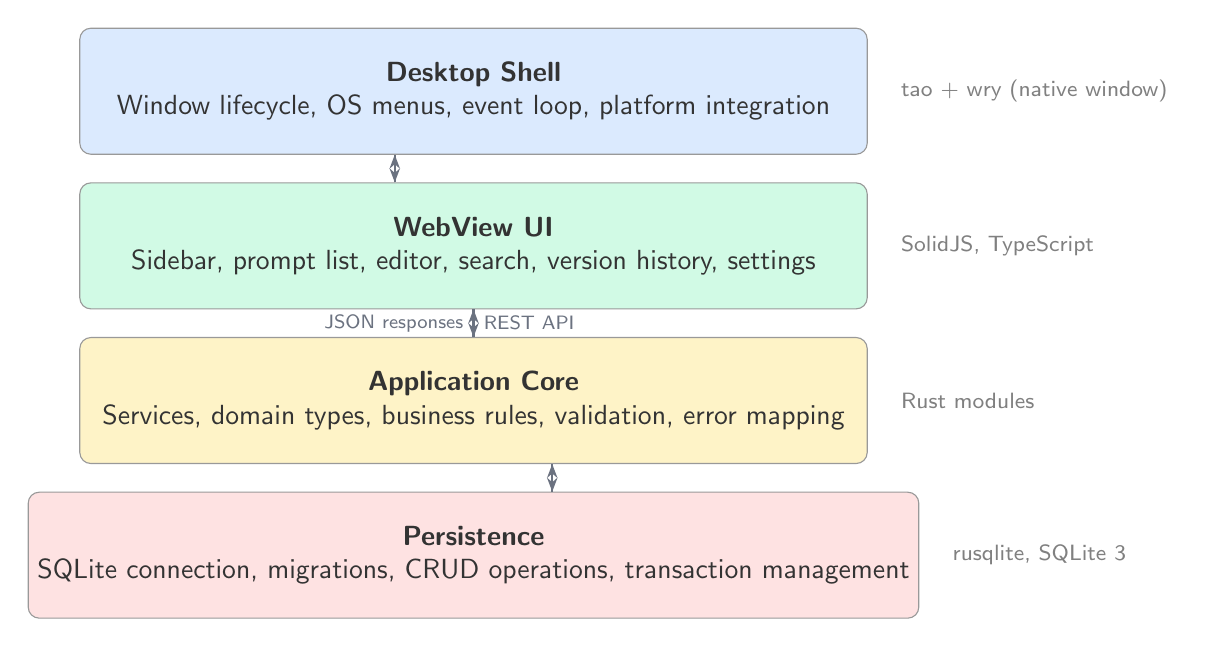
\begin{tikzpicture}[
    layer/.style={
      rectangle,
      draw=black!40,
      rounded corners=4pt,
      minimum width=10cm,
      minimum height=1.6cm,
      font=\sffamily,
      text=black!80,
      align=center
    },
    tech/.style={
      font=\sffamily\footnotesize,
      text=black!50
    },
    arrow/.style={
      -{Stealth[length=5pt]},
      thick,
      color=arrow-gray
    }
  ]
    % Layers from top to bottom
    \node[layer, fill=layer-shell]
      (shell) at (0, 0) {\textbf{Desktop Shell}\\Window lifecycle, OS menus, event loop, platform integration};
    \node[layer, fill=layer-ui, below=0.35cm of shell]
      (ui) {\textbf{WebView UI}\\Sidebar, prompt list, editor, search, version history, settings};
    \node[layer, fill=layer-core, below=0.35cm of ui]
      (core) {\textbf{Application Core}\\Services, domain types, business rules, validation, error mapping};
    \node[layer, fill=layer-db, below=0.35cm of core]
      (db) {\textbf{Persistence}\\SQLite connection, migrations, CRUD operations, transaction management};

    % Technology labels on the right
    \node[tech, right=0.3cm of shell.east, anchor=west] {tao + wry (native window)};
    \node[tech, right=0.3cm of ui.east, anchor=west]    {SolidJS, TypeScript};
    \node[tech, right=0.3cm of core.east, anchor=west]  {Rust modules};
    \node[tech, right=0.3cm of db.east, anchor=west]    {rusqlite, SQLite 3};

    % Bidirectional arrows between layers
    \draw[arrow] (shell.south) +(-1,0) -- +(-1, -0.35) node[midway, left, font=\scriptsize\sffamily, text=arrow-gray] {};
    \draw[arrow] (ui.north)    +(-1,0) -- +(-1,  0.35);

    \draw[arrow] (ui.south)   +(0,0) -- +(0, -0.35) node[midway, right, font=\scriptsize\sffamily, text=arrow-gray] {REST API};
    \draw[arrow] (core.north) +(0,0) -- +(0,  0.35) node[midway, left,  font=\scriptsize\sffamily, text=arrow-gray] {JSON responses};

    \draw[arrow] (core.south) +(1,0) -- +(1, -0.35);
    \draw[arrow] (db.north)   +(1,0) -- +(1,  0.35);
  \end{tikzpicture}
  \caption{Four-layer runtime architecture of NeuronPrompter}
  \label{fig:layers}
\end{figure}

The Desktop Shell layer manages the native window, OS-level menus, and the
application event loop.  It delegates all domain logic downward and never
accesses the database directly.

The WebView UI layer renders the user interface inside a platform-native
WebView component.  It communicates with the Application Core exclusively
through typed IPC commands sent as JSON payloads.

The Application Core contains all business logic: validation, versioning
rules, search coordination, and import/export transformation.  It is the
only layer that orchestrates database transactions.  Clipboard access is a
platform adapter in the Desktop Shell layer; the Application Core triggers
a copy through an abstract interface without depending on any clipboard
library directly.

The Persistence layer encapsulates all SQLite access behind Rust functions
that accept and return domain types.  It owns connection management,
schema migrations, and index definitions.

\section{Technology Stack}
\label{sec:tech-stack}

\Cref{tab:tech-stack} lists every technology and its role in the system.

\begin{table}[H]
  \centering
  \caption{Technology stack}
  \label{tab:tech-stack}
  \begin{tabularx}{\textwidth}{l l X}
    \toprule
    \textbf{Technology} & \textbf{Version} & \textbf{Role} \\
    \midrule
    Rust                & stable (1.88+) & Backend language for all non-UI logic~\cite{rust_book} \\
    axum                & 0.8      & HTTP server framework for the REST API \\
    tao                 & 0.34     & Cross-platform window creation~\cite{tao} \\
    wry                 & 0.54     & WebView rendering abstraction~\cite{wry} \\
    SQLite              & 3.45+    & Embedded relational database~\cite{sqlite} \\
    rusqlite            & 0.32     & Rust bindings for SQLite with bundled build~\cite{rusqlite} \\
    r2d2 / r2d2\_sqlite & 0.8 / 0.25 & Connection pooling for the web server \\
    SolidJS             & latest   & Frontend framework with fine-grained reactivity \\
    TypeScript          & 5.x      & Typed language for frontend logic~\cite{typescript} \\
    serde / serde\_json & 1.x      & Serialization between Rust and JSON~\cite{serde} \\
    anyhow              & 1.x      & Application-level error propagation~\cite{anyhow} \\
    thiserror           & 2.x      & Typed domain error definitions~\cite{thiserror} \\
    tracing             & 0.1.x    & Structured logging and diagnostics~\cite{tracing} \\
    clap                & 4.5      & CLI argument parsing with derive macros \\
    reqwest             & 0.12+    & Async HTTP client for Ollama API calls~\cite{reqwest} \\
    tokio               & 1.x      & Async runtime for axum and reqwest \\
    rust-embed          & 8.x      & Embeds compiled frontend assets into the binary \\
    Vite                & 6.x      & Frontend build toolchain \\
    \bottomrule
  \end{tabularx}
\end{table}

\section{Architecture Decision: axum + tao + wry Instead of Tauri}
\label{sec:adr-framework}

\begin{adrbox}{ADR-1: Use axum + tao + wry directly instead of Tauri}
\textbf{Context.}\quad
The initial design considered using Tauri~2 as an integrated desktop
framework.  An alternative approach uses \texttt{axum} for the HTTP server,
\texttt{tao} for native window management, and \texttt{wry} for WebView
rendering, assembling the application shell from individual components.

\textbf{Decision.}\quad
NeuronPrompter uses \texttt{axum}~0.8 as its REST API server, \texttt{tao}
for the native window event loop, and \texttt{wry} for the embedded WebView.
The frontend communicates with the backend through HTTP REST calls and
Server-Sent Events (SSE), not through Tauri IPC.

\textbf{Rationale.}\quad
Using axum directly provides full control over the HTTP API, enables headless
server mode without framework overhead, and allows the same API to serve both
the embedded WebView and external HTTP clients.  The REST API is testable
without any desktop framework.  Connection pooling via \texttt{r2d2} enables
concurrent request handling.  Cookie-based session authentication and per-IP rate
limiting are implemented as axum middleware.

\textbf{Consequences.}\quad
Packaging, auto-update, and native dialogs must be implemented independently.
The application manages its own window lifecycle through \texttt{tao} and
serves static assets via \texttt{rust-embed}.  In return, the architecture
gains a clean REST boundary that supports headless deployment, MCP child
processes, and future API consumers without framework coupling.
\end{adrbox}

\section{Architecture Decision: Single-Database User Model}
\label{sec:adr-usermodel}

\begin{adrbox}{ADR-2: Store all users in a single SQLite database}
\textbf{Context.}\quad
Two approaches were considered: (A)~a single database file with a
\texttt{user\_id} foreign key on every user-scoped table, and (B)~a
separate database file per user profile.

\textbf{Decision.}\quad
NeuronPrompter uses model~A: one database, all users separated by
\texttt{user\_id}.

\textbf{Rationale.}\quad
A single database file simplifies backup (copy one file), migration
(run one migration script), and application startup (open one connection).
The \texttt{user\_id} column on every scoped table provides logical
isolation.  For the expected data volume (thousands, not millions of
prompts), a single file introduces no measurable performance penalty.

\textbf{Consequences.}\quad
Per-user export requires a filtered query rather than a file copy.  If
physical user isolation becomes necessary later, the schema supports
extraction into per-user databases without structural changes, since
every row already carries its owner's identifier.
\end{adrbox}


\section{Architecture Decision: MCP Server with Dedicated User}
\label{sec:adr-mcp}

\begin{adrbox}{ADR-3: Expose an MCP server with a dedicated database user}
\textbf{Context.}\quad
External AI tools (e.g., Claude Desktop, Cursor) benefit from programmatic
access to the prompt library.  The Model Context Protocol (MCP) defines a
standard interface for this purpose~\cite{mcp_spec}.

\textbf{Decision.}\quad
NeuronPrompter embeds an MCP server that operates under a dedicated
user profile named \texttt{mcp\_agent}.  In headless mode
(\texttt{--mcp}), the server communicates over stdio JSON-RPC.  In
GUI-embedded mode, the server spawns a child-process stdio bridge so
that external tools can connect to the running application.  This profile is auto-created on first activation and
owns its own namespace of prompts, tags, categories, and collections.

\textbf{Rationale.}\quad
A dedicated user profile provides clean isolation between human-authored
and machine-authored prompts.  The MCP user appears in the regular user
list and can be switched to for inspection, but its data does not pollute
the human user's library.  Stdio transport avoids opening network ports
and aligns with the local-first design principle.

\textbf{Consequences.}\quad
The MCP server has full read and write access to the \texttt{mcp\_agent}
namespace.  It does \emph{not} have access to other users' data, Ollama
integration endpoints, or application settings beyond its own user context.
In GUI-embedded mode the server lifecycle is tied to the
application process; in headless mode it runs independently until the
parent closes the stdio pipe.
\end{adrbox}

\section{Architecture Decision: Local Ollama Integration}
\label{sec:adr-ollama}

\begin{adrbox}{ADR-4: Integrate Ollama for local LLM-assisted workflows}
\textbf{Context.}\quad
Users benefit from LLM-assisted features such as prompt improvement,
translation, and automatic metadata derivation (description, language,
notes, tags, and categories).  These operations should run locally without sending
data to cloud services.

\textbf{Decision.}\quad
NeuronPrompter integrates with a locally running Ollama
instance~\cite{ollama} through its HTTP API.  Ollama features are
accessible exclusively through the GUI; the MCP server has no access to
Ollama endpoints.

\textbf{Rationale.}\quad
Ollama provides a standardized HTTP API for local model inference and
supports a wide range of open-weight models.  Restricting Ollama access to
the GUI prevents external tools from triggering expensive inference
operations and keeps the MCP interface focused on data access.  The HTTP
client (\texttt{reqwest}~\cite{reqwest}) communicates with Ollama on
\texttt{localhost:11434} by default; the base URL is configurable per user.

\textbf{Consequences.}\quad
Ollama must be installed and running separately from NeuronPrompter.  If
Ollama is unreachable, the LLM-assisted features degrade gracefully: the
GUI displays an error message and all manual prompt editing remains fully
functional.
\end{adrbox}


\section{Architecture Decision: Layered Error Types}
\label{sec:adr-errors}

\begin{adrbox}{ADR-5: Define error types per crate layer instead of a single
  monolithic error enum}
\textbf{Context.}\quad
The initial design defined a single \texttt{NeuronError} enum in the
\texttt{core} crate with variants for every failure class across all
layers: domain validation, database errors, Ollama HTTP failures,
clipboard access failures, and MCP protocol errors.  This required
\texttt{core} to be aware of infrastructure concerns (database, HTTP,
clipboard) that it has no compile-time dependency on.  Each new
integration added variants to the same enum, creating a cross-layer
knowledge leak.

\textbf{Decision.}\quad
Each crate defines its own error type scoped to the failures that
originate at that layer.  Errors propagate upward through
\texttt{From} trait implementations.

\begin{itemize}
  \item \texttt{CoreError} (\texttt{core}): Validation, NotFound,
        Duplicate.
  \item \texttt{DbError} (\texttt{db}): wraps \texttt{rusqlite::Error}
        and implements \texttt{From<CoreError>}.
  \item \texttt{ServiceError} (\texttt{application}): wraps
        \texttt{DbError}, adds OllamaUnavailable, OllamaError,
        IoError, SerializationError.  Implements
        \texttt{From<DbError>} and \texttt{From<CoreError>}.
  \item \texttt{McpError} (\texttt{mcp}): wraps
        \texttt{ServiceError}, maps to JSON-RPC error codes.
  \item The \texttt{app} crate maps \texttt{ServiceError} variants to
        IPC error codes at the command handler boundary.
\end{itemize}

\textbf{Rationale.}\quad
Layered error types preserve the dependency inversion that the crate
architecture enforces.  \texttt{CoreError} contains no
infrastructure-specific variants, so \texttt{core} remains compilable
and testable without database, HTTP, or platform dependencies.  Adding
a new integration (e.g., a future cloud sync client) adds error
variants to \texttt{ServiceError} without modifying \texttt{CoreError}
or any crate below the application layer.

\textbf{Consequences.}\quad
Error conversions require explicit \texttt{From} implementations at
each crate boundary.  This is a small amount of boilerplate that
\texttt{thiserror}'s \texttt{\#[from]} attribute handles automatically.
Each crate's error type is independently documented and testable.
\end{adrbox}


% =============================================================================
\chapter{Crate Architecture}
\label{ch:crates}
% =============================================================================

\section{Workspace Layout}
\label{sec:workspace}

NeuronPrompter is organized as a Cargo workspace with seven crates.
\Cref{tab:crate-overview} summarizes each crate's responsibility.

\begin{table}[H]
  \centering
  \caption{Cargo workspace crates}
  \label{tab:crate-overview}
  \begin{tabularx}{\textwidth}{l l X}
    \toprule
    \textbf{Crate} & \textbf{Type} & \textbf{Responsibility} \\
    \midrule
    \texttt{neuronprompter-core} & Library &
      Domain types (User, Prompt, Script, Chain, Tag, Collection,
      Category, Version), \texttt{CoreError} for
      domain-level failures, validation rules, template utilities.
      Has zero platform or framework dependencies. \\
    \texttt{neuronprompter-db}   & Library &
      SQLite connection management (single-connection and r2d2
      pool), schema migrations, CRUD operations for all entities,
      full-text search queries.
      Defines \texttt{DbError} wrapping \texttt{rusqlite::Error}.
      Depends on \texttt{neuronprompter-core} for domain types. \\
    \texttt{neuronprompter-application} & Library &
      Service layer: transaction coordination, business rule
      enforcement, versioning workflow, import/export logic,
      Ollama sub-modules (\texttt{client}, \texttt{improve},
      \texttt{translate}, \texttt{metadata}), generic association
      synchronization, script sync, copy service.
      Defines \texttt{ServiceError}.
      Depends on \texttt{neuronprompter-core} and
      \texttt{neuronprompter-db}.  Framework-independent. \\
    \texttt{neuronprompter-mcp}  & Library &
      MCP server implementation: 23 tool definitions, JSON-RPC
      stdio transport, \texttt{mcp\_agent} user management,
      server registration.
      Defines \texttt{McpError} wrapping \texttt{ServiceError}.
      Depends on \texttt{neuronprompter-application} and
      \texttt{neuronprompter-db} for service and database access. \\
    \texttt{neuronprompter-api}  & Library &
      REST API server built on axum: route definitions, HTTP
      handlers for all entities, cookie-based session authentication
      middleware, per-IP rate limiting.
      Defines \texttt{ApiError} mapping \texttt{ServiceError}
      to HTTP status codes.
      Depends on \texttt{neuronprompter-core} for domain types. \\
    \texttt{neuronprompter-web}  & Library &
      Web frontend server: embedded SolidJS SPA via
      \texttt{rust-embed}, SSE event streams, browser launcher,
      native window management (optional \texttt{gui} feature),
      MCP registration and Ollama management endpoints.
      Depends on \texttt{neuronprompter-api} and
      \texttt{neuronprompter-core}. \\
    \texttt{neuronprompter}      & Binary &
      CLI entry point with subcommands: \texttt{web} (GUI mode),
      \texttt{serve} (headless API), \texttt{mcp} (MCP server),
      \texttt{version}.
      Depends on all six library crates. \\
    \bottomrule
  \end{tabularx}
\end{table}

\section{Crate Dependency Diagram}
\label{sec:crate-deps}

\begin{figure}[H]
  \centering
  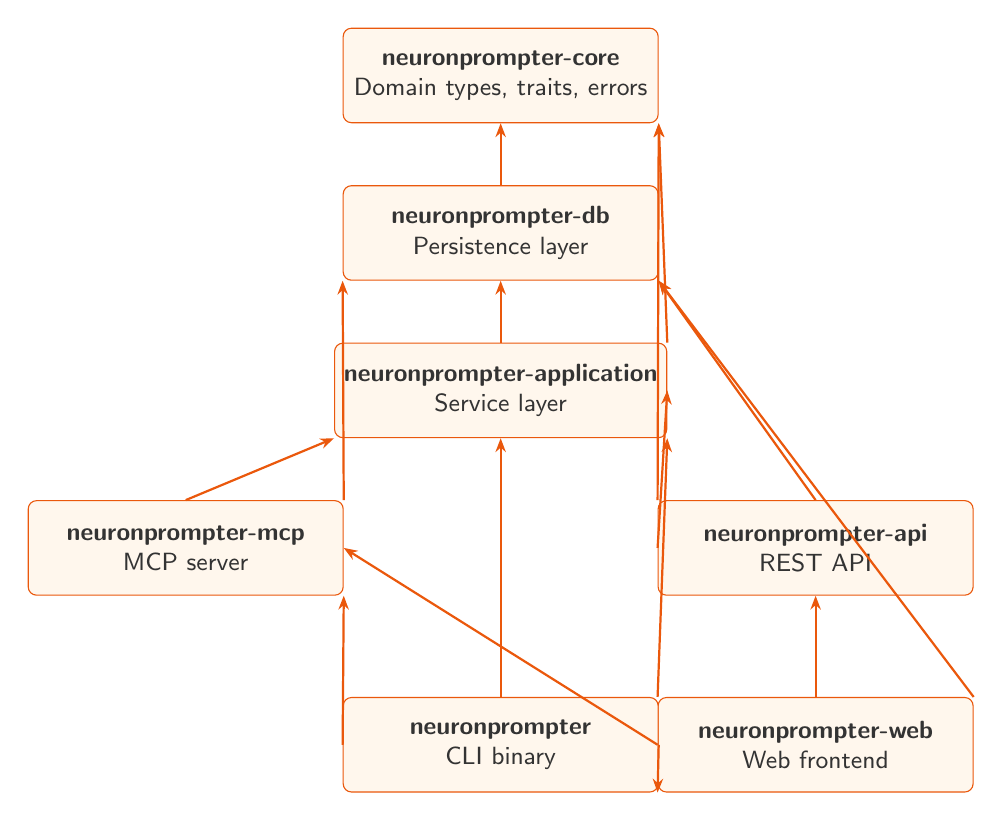
\begin{tikzpicture}[
    crate/.style={
      rectangle,
      draw=crate-border,
      fill=crate-fill,
      rounded corners=3pt,
      minimum width=4cm,
      minimum height=1.2cm,
      font=\sffamily\small,
      text=black!80,
      align=center
    },
    dep/.style={
      -{Stealth[length=5pt]},
      thick,
      color=crate-border
    }
  ]
    \node[crate] (core) at (0, 4)     {\textbf{neuronprompter-core}\\Domain types, traits, errors};
    \node[crate] (db)   at (0, 2)    {\textbf{neuronprompter-db}\\Persistence layer};
    \node[crate] (appl) at (0, 0)    {\textbf{neuronprompter-application}\\Service layer};
    \node[crate] (api)  at (4, -2)   {\textbf{neuronprompter-api}\\REST API};
    \node[crate] (web)  at (4, -4.5) {\textbf{neuronprompter-web}\\Web frontend};
    \node[crate] (mcp)  at (-4, -2)  {\textbf{neuronprompter-mcp}\\MCP server};
    \node[crate] (bin)  at (0, -4.5) {\textbf{neuronprompter}\\CLI binary};

    % db -> core
    \draw[dep] (db.north)    -- (core.south);
    % application -> db, core
    \draw[dep] (appl.north)  -- (db.south);
    \draw[dep] (appl.north east) -- (core.south east);
    % api -> core, application, db
    \draw[dep] (api.north west) -- (core.south east);
    \draw[dep] (api.west) -- (appl.east);
    \draw[dep] (api.north) -- (db.south east);
    % web -> api, application, db, mcp
    \draw[dep] (web.north) -- (api.south);
    \draw[dep] (web.north west) -- (appl.south east);
    \draw[dep] (web.west) -- (mcp.east);
    \draw[dep] (web.north east) -- (db.south east);
    % mcp -> application, db
    \draw[dep] (mcp.north)   -- (appl.south west);
    \draw[dep] (mcp.north east) -- (db.south west);
    % bin -> mcp, web, appl
    \draw[dep] (bin.north) -- (appl.south);
    \draw[dep] (bin.west) -- (mcp.south east);
    \draw[dep] (bin.east) -- (web.south west);
  \end{tikzpicture}
  \caption{Crate dependency graph (transitive reduction).  Arrows point from dependent to dependency.}
  \label{fig:crate-deps}
\end{figure}

The \texttt{neuronprompter-core} crate sits at the top of the dependency
tree and has no knowledge of SQLite, axum, MCP, or any framework.  Its
\texttt{CoreError} type contains only domain-level failure variants;
infrastructure errors are defined in the crates that own the respective
dependencies (see \cref{sec:adr-errors}).  This isolation guarantees
that domain logic can be tested without a database or windowing system.

The \texttt{neuronprompter-application} crate contains the service layer:
business rule enforcement, transaction coordination, versioning workflow,
import/export logic, and the Ollama sub-modules (\texttt{client},
\texttt{improve}, \texttt{translate}, \texttt{metadata}).  It depends on
\texttt{core} for domain types, \texttt{db} for persistence, and
\texttt{reqwest} for async HTTP communication with Ollama.  It has no
dependency on axum, MCP, or any UI framework.

The \texttt{neuronprompter-api} crate provides the REST API layer built
on axum, with HTTP handlers, cookie-based session authentication middleware, and
per-IP rate limiting.  It depends on \texttt{core} for domain types.

The \texttt{neuronprompter-web} crate extends the API router with web-specific
endpoints: embedded SPA serving via \texttt{rust-embed}, SSE log and model
event streams, browser launcher, and optional native window management
(\texttt{gui} feature with \texttt{tao}~+~\texttt{wry}).

All consumer crates route through the service layer (all crate names
carry the \texttt{neuronprompter-} prefix):

\begin{itemize}
  \item REST API path: \texttt{api} $\to$ \texttt{application} $\to$ \texttt{db}
  \item Web path: \texttt{web} $\to$ \texttt{api} $\to$ \texttt{application} $\to$ \texttt{db}
  \item MCP path: \texttt{mcp} $\to$ \texttt{application} $\to$ \texttt{db}
\end{itemize}

This guarantees that validation, versioning, and side effects are enforced
uniformly regardless of whether a request originates from the REST API, the
web UI, or an MCP client.

\section{Module Breakdown: neuronprompter-core}
\label{sec:mod-core}

\begin{table}[H]
  \centering
  \caption{Modules in \texttt{neuronprompter-core}}
  \label{tab:mod-core}
  \begin{tabularx}{\textwidth}{l l X}
    \toprule
    \textbf{Module path} & \textbf{File} & \textbf{Contents} \\
    \midrule
    \texttt{lib}           & \texttt{lib.rs}       & Crate root, public re-exports \\
    \texttt{domain}        & \texttt{domain/mod.rs}& Domain module root, re-exports all entity types \\
    \texttt{domain::user}  & \texttt{domain/user.rs}      & \texttt{User} struct, \texttt{NewUser} input type \\
    \texttt{domain::prompt}& \texttt{domain/prompt.rs}    & \texttt{Prompt}, \texttt{NewPrompt}, \texttt{UpdatePrompt} \\
    \texttt{domain::script}& \texttt{domain/script.rs}    & \texttt{Script}, \texttt{NewScript}, \texttt{UpdateScript} \\
    \texttt{domain::script\_version} & \texttt{domain/script\_version.rs} & \texttt{ScriptVersion} \\
    \texttt{domain::chain} & \texttt{domain/chain.rs}     & \texttt{Chain}, \texttt{ChainStep}, \texttt{NewChain} \\
    \texttt{domain::tag}   & \texttt{domain/tag.rs}       & \texttt{Tag}, \texttt{NewTag} \\
    \texttt{domain::collection} & \texttt{domain/collection.rs} & \texttt{Collection}, \texttt{NewCollection} \\
    \texttt{domain::category}   & \texttt{domain/category.rs}   & \texttt{Category}, \texttt{NewCategory} \\
    \texttt{domain::version}    & \texttt{domain/version.rs}    & \texttt{PromptVersion} \\
    \texttt{domain::settings}   & \texttt{domain/settings.rs}   & \texttt{AppSetting} key-value pair,
                                                            \texttt{UserSettings} struct \\
    \texttt{error}         & \texttt{error.rs}     & \texttt{CoreError} enum with \texttt{thiserror}
                                                      derivation.  Covers domain-level failures
                                                      (validation, not found, duplicate, entity in use,
                                                      authorization, path traversal, conflict) \\
    \texttt{paths}         & \texttt{paths.rs}     & Filesystem sandboxing and path utilities \\
    \texttt{serde\_helpers} & \texttt{serde\_helpers.rs} & Custom serde deserializer for
                                                      \texttt{Option<Option<T>{}>} fields,
                                                      distinguishing absent from explicit null \\
    \texttt{constants}     & \texttt{constants.rs} & Shared constants (default Ollama URL, default port) \\
    \texttt{template}      & \texttt{template.rs}  & Template variable detection and rendering \\
    \texttt{validation}    & \texttt{validation.rs}& Input validation rules (title, username,
                                                      language code, content, separator) \\
    \bottomrule
  \end{tabularx}
\end{table}

\section{Module Breakdown: neuronprompter-db}
\label{sec:mod-db}

\begin{table}[H]
  \centering
  \caption{Modules in \texttt{neuronprompter-db}}
  \label{tab:mod-db}
  \begin{tabularx}{\textwidth}{l l X}
    \toprule
    \textbf{Module path} & \textbf{File} & \textbf{Contents} \\
    \midrule
    \texttt{lib}              & \texttt{lib.rs}          & Crate root, public API \\
    \texttt{connection}       & \texttt{connection.rs}   & \texttt{Database} struct, single-connection
                                                           wrapper for MCP compatibility, WAL configuration \\
    \texttt{connection\_provider} & \texttt{connection\_provider.rs} & \texttt{ConnectionProvider} trait
                                                           abstracting over \texttt{Database} and \texttt{DbPool} \\
    \texttt{pool}             & \texttt{pool.rs}         & r2d2 connection pool for the web server,
                                                           \texttt{DbPool} and \texttt{PooledConn} types \\
    \texttt{migrations}       & \texttt{migrations.rs}   & Schema version tracking, forward-only
                                                           migration execution \\
    \texttt{error}            & \texttt{error.rs}        & \texttt{DbError} wrapping \texttt{rusqlite::Error} \\
    \texttt{repo}             & \texttt{repo/mod.rs}     & Repository module root, re-exports \\
    \texttt{repo::users}      & \texttt{repo/users.rs}        & CRUD for the \texttt{users} table \\
    \texttt{repo::prompts}    & \texttt{repo/prompts.rs}      & CRUD for \texttt{prompts}, filtered queries \\
    \texttt{repo::scripts}    & \texttt{repo/scripts.rs}      & CRUD for \texttt{scripts}, filesystem sync queries \\
    \texttt{repo::script\_versions} & \texttt{repo/script\_versions.rs} & Insert and query \texttt{script\_versions} \\
    \texttt{repo::chains}     & \texttt{repo/chains.rs}       & CRUD for \texttt{chains} and \texttt{chain\_steps} \\
    \texttt{repo::tags}       & \texttt{repo/tags.rs}         & CRUD for \texttt{tags} and tag junction tables \\
    \texttt{repo::collections}& \texttt{repo/collections.rs}  & CRUD for \texttt{collections} and
                                                           collection junction tables \\
    \texttt{repo::categories} & \texttt{repo/categories.rs}   & CRUD for \texttt{categories} and
                                                           category junction tables \\
    \texttt{repo::versions}   & \texttt{repo/versions.rs}     & Insert and query \texttt{prompt\_versions} \\
    \texttt{repo::settings}   & \texttt{repo/settings.rs}     & Read/write \texttt{app\_settings} and
                                                           \texttt{user\_settings} \\
    \texttt{repo::search}     & \texttt{repo/search.rs}       & Full-text search queries (FTS5) for
                                                           prompts, scripts, and chains \\
    \bottomrule
  \end{tabularx}
\end{table}

\section{Module Breakdown: neuronprompter-api}
\label{sec:mod-api}

{\footnotesize
\begin{longtable}{L{4cm} L{4.8cm} L{5.8cm}}
  \caption{Modules in \texttt{neuronprompter-api}}
  \label{tab:mod-api} \\
  \toprule
  \textbf{Module path} & \textbf{File} & \textbf{Contents} \\
  \midrule
  \endfirsthead
  \toprule
  \textbf{Module path} & \textbf{File} & \textbf{Contents} \\
  \midrule
  \endhead
  \texttt{lib}                    & \texttt{lib.rs}                 & Crate root, public API exports \\
  \texttt{router}                 & \texttt{router.rs}              & Route definitions, \texttt{build\_router} function \\
  \texttt{state}                  & \texttt{state.rs}               & \texttt{AppState} with db pool, Ollama client,
                                                                      session management \\
  \texttt{error}                  & \texttt{error.rs}               & \texttt{ApiError} with HTTP status mapping \\
  \texttt{handlers}               & \texttt{handlers/mod.rs}        & Handler module root, re-exports \\
  \texttt{handlers::common}       & \texttt{handlers/common.rs}     & Shared handler utilities (IO path validation) \\
  \texttt{handlers::health}       & \texttt{handlers/health.rs}     & Health check and database path endpoints \\
  \texttt{handlers::shutdown}     & \texttt{handlers/shutdown.rs}   & Graceful shutdown endpoint \\
  \texttt{handlers::users}        & \texttt{handlers/users.rs}      & User CRUD handlers \\
  \texttt{handlers::prompts}      & \texttt{handlers/prompts.rs}    & Prompt CRUD handlers \\
  \texttt{handlers::scripts}      & \texttt{handlers/scripts.rs}    & Script CRUD handlers \\
  \texttt{handlers::chains}       & \texttt{handlers/chains.rs}     & Chain CRUD and composition handlers \\
  \texttt{handlers::copy}         & \texttt{handlers/copy.rs}       & Cross-user copy handlers \\
  \texttt{handlers::tags}         & \texttt{handlers/tags.rs}       & Tag CRUD handlers \\
  \texttt{handlers::collections}  & \texttt{handlers/collections.rs}& Collection CRUD handlers \\
  \texttt{handlers::categories}   & \texttt{handlers/categories.rs} & Category CRUD handlers \\
  \texttt{handlers::versions}     & \texttt{handlers/versions.rs}   & Prompt version handlers \\
  \texttt{handlers::script\_\-versions} & \texttt{handlers/script\_versions.rs} & Script version handlers \\
  \texttt{handlers::search}       & \texttt{handlers/search.rs}     & Full-text search handlers \\
  \texttt{handlers::io}           & \texttt{handlers/io.rs}         & Import, export, backup handlers \\
  \texttt{handlers::clipboard}    & \texttt{handlers/clipboard.rs}  & Copy-to-clipboard handler \\
  \texttt{handlers::settings}     & \texttt{handlers/settings.rs}   & App and user settings handlers \\
  \texttt{handlers::ollama}       & \texttt{handlers/ollama.rs}     & Ollama LLM operation handlers \\
  \texttt{handlers::sessions}    & \texttt{handlers/sessions.rs}   & Session login, switch, logout, status endpoints \\
  \texttt{session}               & \texttt{session.rs}             & In-memory session store (DashMap, CSPRNG tokens, TTL, LRU eviction) \\
  \texttt{middleware}             & \texttt{middleware/mod.rs}       & Middleware module root \\
  \texttt{middleware::auth}       & \texttt{middleware/auth.rs}      & Ownership and user-param verification \\
  \texttt{middleware::session}    & \texttt{middleware/session.rs}   & Cookie-based session middleware, AuthUser/AuthSession extractors \\
  \texttt{middleware::rate\_limit}& \texttt{middleware/rate\_limit.rs} & Per-IP rate limiting (dashmap) \\
  \texttt{tests}                & \texttt{tests.rs}               & Handler integration tests \\
  \bottomrule
\end{longtable}
}

\section{Module Breakdown: neuronprompter-web}
\label{sec:mod-web}

{\footnotesize
\begin{longtable}{L{4cm} L{4.8cm} L{5.8cm}}
  \caption{Modules in \texttt{neuronprompter-web}}
  \label{tab:mod-web} \\
  \toprule
  \textbf{Module path} & \textbf{File} & \textbf{Contents} \\
  \midrule
  \endfirsthead
  \toprule
  \textbf{Module path} & \textbf{File} & \textbf{Contents} \\
  \midrule
  \endhead
  \texttt{lib}                    & \texttt{lib.rs}              & Crate root, \texttt{WebState}, \texttt{build\_web\_router} \\
  \texttt{assets}                 & \texttt{assets.rs}           & Embedded SPA serving via \texttt{rust-embed},
                                                                    SPA fallback routing \\
  \texttt{broadcast\_layer}       & \texttt{broadcast\_layer.rs} & Tracing layer forwarding logs via SSE \\
  \texttt{browser}                & \texttt{browser.rs}          & Cross-platform browser launcher \\
  \texttt{sse}                    & \texttt{sse.rs}              & Server-Sent Event endpoints for logs
                                                                    and model events \\
  \texttt{handlers}               & \texttt{handlers/mod.rs}     & Web-specific handler module root \\
  \texttt{handlers::setup}        & \texttt{handlers/setup.rs}   & First-run setup status and completion \\
  \texttt{handlers::doctor}       & \texttt{handlers/doctor.rs}  & System health probes \\
  \texttt{handlers::mcp}          & \texttt{handlers/mcp.rs}     & MCP registration install/uninstall \\
  \texttt{handlers::ollama}       & \texttt{handlers/ollama.rs}  & Ollama model management (list, pull, delete) \\
  \texttt{handlers::dialogs}      & \texttt{handlers/dialogs.rs} & Native file dialog endpoints (gui feature) \\
  \texttt{native\_window}         & \texttt{native\_window.rs}   & Native window management via tao + wry
                                                                    (feature-gated: \texttt{gui}) \\
  \texttt{splash}                 & \texttt{splash.rs}           & Splash screen rendering
                                                                    (feature-gated: \texttt{gui}) \\
  \texttt{tests}                  & \texttt{tests.rs}            & SSE and web handler tests \\
  \bottomrule
\end{longtable}
}

\section{Module Breakdown: neuronprompter (binary)}
\label{sec:mod-bin}

\begin{table}[H]
  \centering
  \caption{Modules in \texttt{neuronprompter} (binary crate)}
  \label{tab:mod-bin}
  \begin{tabularx}{\textwidth}{l l X}
    \toprule
    \textbf{Module path} & \textbf{File} & \textbf{Contents} \\
    \midrule
    \texttt{main}               & \texttt{main.rs}           & CLI entry point with clap-derived subcommands:
                                                               \texttt{web} (GUI mode with browser/native
                                                               window), \texttt{serve} (headless API server),
                                                               \texttt{mcp} (MCP server operations),
                                                               \texttt{version} (print version).
                                                               Default features: \texttt{web}, \texttt{gui},
                                                               \texttt{mcp} \\
    \bottomrule
  \end{tabularx}
\end{table}

\begin{table}[H]
  \centering
  \caption{Feature flag definitions}
  \label{tab:features}
  \begin{tabularx}{\textwidth}{l l l X}
    \toprule
    \textbf{Crate} & \textbf{Feature} & \textbf{Default} & \textbf{Description} \\
    \midrule
    \texttt{neuronprompter} & \texttt{web} & yes & Enables the web UI subcommand with browser launcher \\
    \texttt{neuronprompter} & \texttt{gui} & yes & Enables native window management (tao + wry) \\
    \texttt{neuronprompter} & \texttt{mcp} & yes & Enables the MCP server subcommand \\
    \texttt{neuronprompter-web} & \texttt{gui} & yes & Enables native window, splash screen, and file dialogs \\
    \bottomrule
  \end{tabularx}
\end{table}

\section{Module Breakdown: neuronprompter-application}
\label{sec:mod-application}

{\footnotesize
\begin{longtable}{L{4cm} L{4.8cm} L{5.8cm}}
  \caption{Modules in \texttt{neuronprompter-application}}
  \label{tab:mod-application} \\
  \toprule
  \textbf{Module path} & \textbf{File} & \textbf{Contents} \\
  \midrule
  \endfirsthead
  \toprule
  \textbf{Module path} & \textbf{File} & \textbf{Contents} \\
  \midrule
  \endhead
  \texttt{lib}               & \texttt{lib.rs}          & Crate root, public service API \\
  \texttt{error}             & \texttt{error.rs}        & \texttt{ServiceError} wrapping \texttt{DbError}
                                                           and adding HTTP/IO variants \\
  \texttt{prompt\_service}   & \texttt{prompt\_service.rs} & Prompt CRUD with validation.  Delegates
                                                             versioning steps to \texttt{version\_service}
                                                             and association updates to
                                                             \texttt{association\_sync} \\
  \texttt{script\_service}   & \texttt{script\_service.rs} & Script CRUD with filesystem sync support \\
  \texttt{script\_version\_service} & \texttt{script\_version\_service.rs} & Script versioning:
                                                             snapshot creation, version counter,
                                                             history queries, version restore \\
  \texttt{chain\_service}    & \texttt{chain\_service.rs}  & Chain CRUD, step management,
                                                             composed content generation, duplication \\
  \texttt{version\_service}  & \texttt{version\_service.rs}& Prompt versioning logic: snapshot creation,
                                                             version counter management, history
                                                             queries, version restore \\
  \texttt{association\_sync} & \texttt{association\_sync.rs}& Generic helper for synchronizing
                                                             many-to-many associations for tags,
                                                             categories, and collections.  Used by
                                                             prompt, script, and chain services \\
  \texttt{user\_service}     & \texttt{user\_service.rs}   & User creation, deletion with cascade,
                                                             profile switching \\
  \texttt{tag\_service}      & \texttt{tag\_service.rs}    & Tag lifecycle and entity-tag association \\
  \texttt{category\_service} & \texttt{category\_service.rs} & Category lifecycle and entity-category
                                                                association \\
  \texttt{collection\_service} & \texttt{collection\_service.rs} & Collection lifecycle and
                                                                    entity-collection association \\
  \texttt{copy\_service}     & \texttt{copy\_service.rs}   & Cross-user copying of prompts, scripts,
                                                             and chains with taxonomy transfer \\
  \texttt{search\_service}   & \texttt{search\_service.rs} & Search coordination: assembles FTS5
                                                              queries for prompts, scripts, and chains,
                                                              enforces result limit \\
  \texttt{sync\_service}     & \texttt{sync\_service.rs}   & Filesystem synchronization for scripts:
                                                              import from file, detect external changes \\
  \texttt{settings\_service} & \texttt{settings\_service.rs} & App-wide and per-user settings management \\
  \texttt{io\_service}       & \texttt{io\_service.rs}     & JSON and Markdown import/export with source
                                                                user envelope, database backup \\
  \texttt{ollama}            & \texttt{ollama/mod.rs}       & Sub-module root, re-exports the public
                                                             service facade \\
  \texttt{ollama::client}    & \texttt{ollama/client.rs}    & HTTP client for the Ollama API:
                                                             connection management, health check
                                                             (\texttt{/api/tags}), and the generic
                                                             \texttt{/api/generate} request function \\
  \texttt{ollama::improve}   & \texttt{ollama/improve.rs}   & Improvement workflow: system prompt
                                                             template, request construction,
                                                             response parsing \\
  \texttt{ollama::translate} & \texttt{ollama/translate.rs}  & Translation workflow: system prompt
                                                             template, target language handling,
                                                             response parsing \\
  \texttt{ollama::metadata}  & \texttt{ollama/metadata.rs}  & Metadata derivation workflow: decomposed
                                                             plain-text extraction for \texttt{description},
                                                             \texttt{language}, \texttt{notes}, \texttt{suggested\_tags},
                                                             and \texttt{suggested\_categories}
                                                             (see \cref{sec:ollama-templates}) \\
  \bottomrule
\end{longtable}
}

\section{Module Breakdown: neuronprompter-mcp}
\label{sec:mod-mcp}

\begin{table}[H]
  \centering
  \caption{Modules in \texttt{neuronprompter-mcp}}
  \label{tab:mod-mcp}
  \begin{tabularx}{\textwidth}{l l X}
    \toprule
    \textbf{Module path} & \textbf{File} & \textbf{Contents} \\
    \midrule
    \texttt{lib}              & \texttt{lib.rs}              & Crate root, public API, \texttt{run\_stdio\_server} \\
    \texttt{server}           & \texttt{server.rs}           & JSON-RPC 2.0 stdio server lifecycle \\
    \texttt{transport}        & \texttt{transport.rs}        & Stdin/stdout message framing \\
    \texttt{tools}            & \texttt{tools.rs}            & 23 tool definitions and dispatch via \texttt{\#[tool\_router]}
                                                                macro (prompts~5, scripts~5, chains~8, tags~2,
                                                                categories~2, collections~1) \\
    \texttt{tool\_prompts}    & \texttt{tool\_prompts.rs}    & Reserved stub module \\
    \texttt{tool\_tags}       & \texttt{tool\_tags.rs}       & Reserved stub module \\
    \texttt{tool\_categories} & \texttt{tool\_categories.rs} & Reserved stub module \\
    \texttt{auth}             & \texttt{auth.rs}             & \texttt{mcp\_agent} user creation and validation \\
    \texttt{registration}     & \texttt{registration.rs}     & MCP server registration in Claude config \\
    \texttt{error}            & \texttt{error.rs}            & \texttt{McpError} with JSON-RPC code mapping \\
    \bottomrule
  \end{tabularx}
\end{table}

\section{Workspace Directory Structure}
\label{sec:dir-structure}

The following table maps logical components to their file system locations
relative to the workspace root.

\begin{table}[H]
  \centering
  \caption{Top-level directory layout}
  \label{tab:dir-layout}
  \begin{tabularx}{\textwidth}{l X}
    \toprule
    \textbf{Path} & \textbf{Purpose} \\
    \midrule
    \texttt{Cargo.toml}            & Workspace manifest listing all seven member crates \\
    \texttt{crates/neuronprompter-core/}          & \texttt{neuronprompter-core} library crate \\
    \texttt{crates/neuronprompter-core/src/domain/} & Domain types: user, prompt, script, chain,
                                       tag, collection, category, version, settings \\
    \texttt{crates/neuronprompter-core/src/serde\_helpers.rs} & Custom serde deserializer for
                                       \texttt{Option<Option<T>{}>} (absent vs.\ null distinction) \\
    \texttt{crates/neuronprompter-db/}            & \texttt{neuronprompter-db} library crate \\
    \texttt{crates/neuronprompter-db/src/repo/}   & Repository modules: one per entity \\
    \texttt{crates/neuronprompter-application/}   & \texttt{neuronprompter-application} library crate
                                     (service layer) \\
    \texttt{crates/neuronprompter-application/src/ollama/} & Ollama sub-modules: \texttt{client.rs},
                                              \texttt{improve.rs}, \texttt{translate.rs},
                                              \texttt{metadata.rs} \\
    \texttt{crates/neuronprompter-api/}           & \texttt{neuronprompter-api} library crate (REST API) \\
    \texttt{crates/neuronprompter-api/src/handlers/} & HTTP handlers: one per entity \\
    \texttt{crates/neuronprompter-api/src/middleware/} & Authentication and rate limiting \\
    \texttt{crates/neuronprompter-web/}           & \texttt{neuronprompter-web} library crate (web server) \\
    \texttt{crates/neuronprompter-web/src/handlers/} & Web-specific handlers (setup, doctor, mcp, ollama,
                                        dialogs) \\
    \texttt{crates/neuronprompter-web/frontend/}  & SolidJS + TypeScript + Vite project \\
    \texttt{crates/neuronprompter-mcp/}           & \texttt{neuronprompter-mcp} library crate (MCP server) \\
    \texttt{crates/neuronprompter/}               & \texttt{neuronprompter} binary crate (CLI entry) \\
    \texttt{docs/}                 & This architecture document and bibliography \\
    \texttt{migrations/}           & SQL migration files, numbered sequentially \\
    \texttt{tools/ci/}             & CI validation scripts (schema, architecture, tests) \\
    \texttt{tools/gen/}            & Code generation utilities (diagrams, test chapters) \\
    \texttt{.githooks/}            & Git hook scripts (pre-commit validation) \\
    \bottomrule
  \end{tabularx}
\end{table}

\section{Application State}
\label{sec:app-state}

The REST API server uses an \texttt{AppState} struct (defined in
\texttt{neuronprompter-api}) that holds the database connection pool,
Ollama HTTP client, and session management.  This state is passed
to all axum handlers via the \texttt{State} extractor.

The web server extends this with a \texttt{WebState} struct (defined in
\texttt{neuronprompter-web}) that adds SSE broadcast channels for log
and model events, an SSE connection counter, and a flag for native
file dialog support.

In MCP mode, the server uses a single \texttt{Database} connection
(not a pool) since MCP child processes handle one request at a time
over stdio.


% =============================================================================
\chapter{Data Architecture}
\label{ch:data}
% =============================================================================

\section{Storage Strategy}
\label{sec:storage-strategy}

NeuronPrompter stores all persistent data in a single SQLite database file
located in the OS-standard application data directory (see
\cref{sec:fs-paths}).  The database connection is opened at application
startup with the following pragmas applied immediately:

\begin{table}[H]
  \centering
  \caption{SQLite connection pragmas}
  \label{tab:pragmas}
  \begin{tabularx}{\textwidth}{l l X}
    \toprule
    \textbf{Pragma} & \textbf{Value} & \textbf{Effect} \\
    \midrule
    \texttt{journal\_mode} & WAL    & Allows concurrent reads during writes,
                                       reduces lock contention~\cite{sqlite} \\
    \texttt{foreign\_keys}  & ON     & Enforces referential integrity at the
                                       database engine level \\
    \texttt{synchronous}    & NORMAL & Balances durability and write speed;
                                       acceptable for a local desktop application
                                       where OS-level crashes are rare \\
    \texttt{busy\_timeout}  & 5000   & Waits up to 5 seconds for a locked
                                       database before returning an error \\
    \bottomrule
  \end{tabularx}
\end{table}

\section{Entity-Relationship Diagram}
\label{sec:er-diagram}

\Cref{fig:er} shows the relationships between all database entities.

\begin{figure}[H]
  \centering
  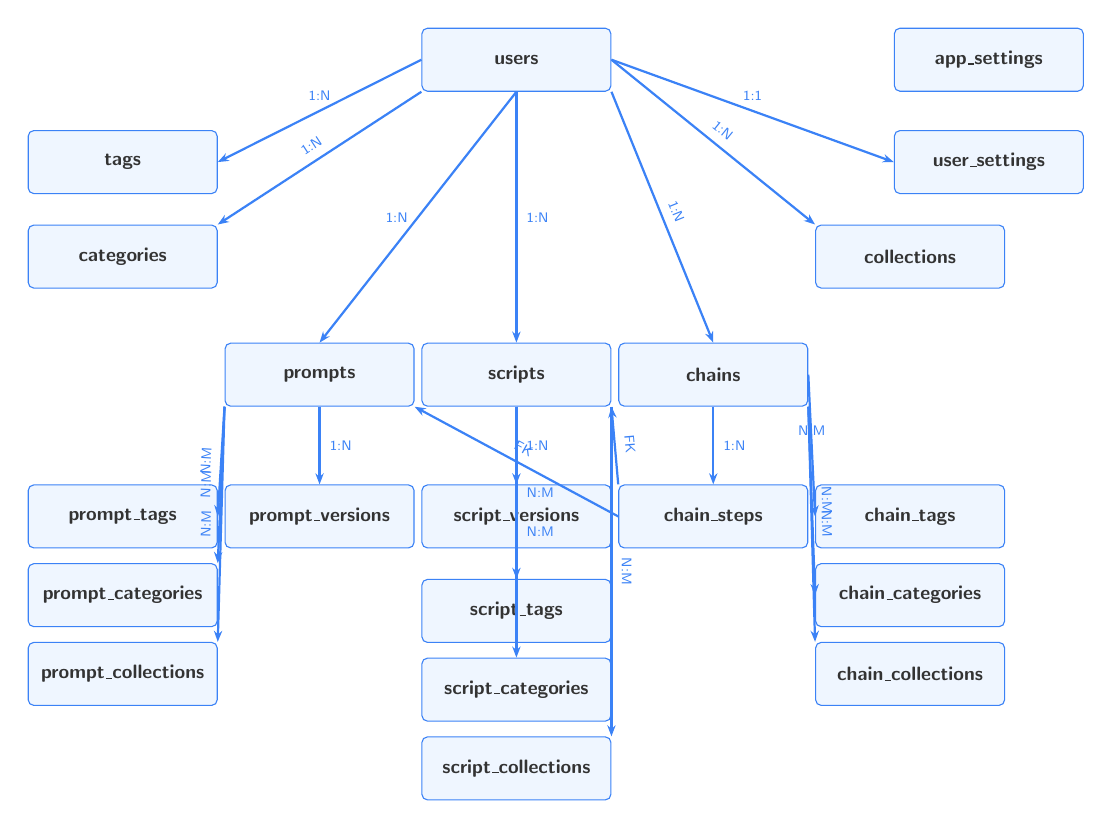
\begin{tikzpicture}[
    entity/.style={
      rectangle,
      draw=entity-border,
      fill=entity-fill,
      rounded corners=2pt,
      minimum width=2.4cm,
      minimum height=0.8cm,
      font=\sffamily\scriptsize,
      text=black!80,
      align=center
    },
    rel/.style={
      -{Stealth[length=4pt]},
      thick,
      color=entity-border
    },
    card/.style={
      font=\sffamily\tiny,
      text=entity-border
    }
  ]
    % ---- Top row: users, settings ----
    \node[entity] (users)        at (0, 0)       {\textbf{users}};
    \node[entity] (settings)     at (6, 0)       {\textbf{app\_settings}};
    \node[entity] (usettings)    at (6, -1.3)    {\textbf{user\_settings}};

    % ---- Taxonomy row ----
    \node[entity] (tags)         at (-5, -1.3)   {\textbf{tags}};
    \node[entity] (categories)   at (-5, -2.5)   {\textbf{categories}};
    \node[entity] (collections)  at (5, -2.5)    {\textbf{collections}};

    % ---- Content entities row ----
    \node[entity] (prompts)      at (-2.5, -4)   {\textbf{prompts}};
    \node[entity] (scripts)      at (0, -4)      {\textbf{scripts}};
    \node[entity] (chains)       at (2.5, -4)    {\textbf{chains}};

    % ---- Version tables ----
    \node[entity] (pversions)    at (-2.5, -5.8) {\textbf{prompt\_versions}};
    \node[entity] (sversions)    at (0, -5.8)    {\textbf{script\_versions}};
    \node[entity] (csteps)       at (2.5, -5.8)  {\textbf{chain\_steps}};

    % ---- Prompt junction tables ----
    \node[entity] (pt)           at (-5, -5.8)   {\textbf{prompt\_tags}};
    \node[entity] (pcat)         at (-5, -6.8)   {\textbf{prompt\_categories}};
    \node[entity] (pcol)         at (-5, -7.8)   {\textbf{prompt\_collections}};

    % ---- Script junction tables ----
    \node[entity] (st)           at (0, -7)      {\textbf{script\_tags}};
    \node[entity] (scat)         at (0, -8)      {\textbf{script\_categories}};
    \node[entity] (scol)         at (0, -9)      {\textbf{script\_collections}};

    % ---- Chain junction tables ----
    \node[entity] (ct)           at (5, -5.8)    {\textbf{chain\_tags}};
    \node[entity] (ccat)         at (5, -6.8)    {\textbf{chain\_categories}};
    \node[entity] (ccol)         at (5, -7.8)    {\textbf{chain\_collections}};

    % ---- Users -> content entities ----
    \draw[rel] (users.south) -- (prompts.north)
      node[card, midway, left] {1:N};
    \draw[rel] (users.south) -- (scripts.north)
      node[card, midway, right] {1:N};
    \draw[rel] (users.south east) -- (chains.north)
      node[card, midway, above, sloped] {1:N};

    % ---- Users -> taxonomy ----
    \draw[rel] (users.west) -- (tags.east)
      node[card, midway, above] {1:N};
    \draw[rel] (users.south west) -- (categories.north east)
      node[card, midway, above, sloped] {1:N};
    \draw[rel] (users.east) -- (collections.north west)
      node[card, midway, above, sloped] {1:N};
    \draw[rel] (users.east) -- (usettings.west)
      node[card, midway, above] {1:1};

    % ---- Content -> versions ----
    \draw[rel] (prompts.south) -- (pversions.north)
      node[card, midway, right] {1:N};
    \draw[rel] (scripts.south) -- (sversions.north)
      node[card, midway, right] {1:N};
    \draw[rel] (chains.south) -- (csteps.north)
      node[card, midway, right] {1:N};

    % ---- Prompt junction ----
    \draw[rel] (prompts.south west) -- (pt.east)
      node[card, midway, above, sloped] {N:M};
    \draw[rel] (prompts.south west) -- (pcat.north east)
      node[card, midway, above, sloped] {N:M};
    \draw[rel] (prompts.south west) -- (pcol.north east)
      node[card, midway, above, sloped] {N:M};

    % ---- Script junction ----
    \draw[rel] (scripts.south) -- (st.north)
      node[card, midway, right] {N:M};
    \draw[rel] (scripts.south) -- (scat.north)
      node[card, midway, right] {N:M};
    \draw[rel] (scripts.south east) -- (scol.north east)
      node[card, midway, above, sloped] {N:M};

    % ---- Chain junction ----
    \draw[rel] (chains.east) -- (ct.west)
      node[card, midway, above] {N:M};
    \draw[rel] (chains.south east) -- (ccat.west)
      node[card, midway, above, sloped] {N:M};
    \draw[rel] (chains.south east) -- (ccol.north west)
      node[card, midway, above, sloped] {N:M};

    % ---- Chain steps -> prompts/scripts ----
    \draw[rel] (csteps.west) -- (prompts.south east)
      node[card, midway, above, sloped] {FK};
    \draw[rel] (csteps.north west) -- (scripts.south east)
      node[card, midway, above, sloped] {FK};
  \end{tikzpicture}
  \caption{Entity-relationship diagram.  Prompts, scripts, and chains
           each have dedicated junction tables for tags, categories, and
           collections (many-to-many).  Chain steps reference prompts
           and/or scripts.  \texttt{user\_settings} has a 1:1 relationship
           with \texttt{users}.}
  \label{fig:er}
\end{figure}

\section{Entity: users}
\label{sec:entity-users}

Stores local user profiles.  Each profile owns prompts, tags, and
collections through a foreign key relationship.

\textbf{Important:} User profiles are convenience profiles, not security
accounts.  There is no password, no encryption boundary, and no access
control between profiles.  Any user of the operating system account that
runs NeuronPrompter can switch to any profile and read all data.  The
profile system exists to separate prompt libraries on a shared workstation,
not to enforce confidentiality.

\begin{table}[H]
  \centering
  \caption{Schema: \texttt{users}}
  \label{tab:schema-users}
  \begin{tabularx}{\textwidth}{l l l X}
    \toprule
    \textbf{Column} & \textbf{Type} & \textbf{Constraints} & \textbf{Description} \\
    \midrule
    id            & INTEGER & PK, autoincrement & Surrogate primary key \\
    username      & TEXT    & NOT NULL, UNIQUE   & Login-style identifier, lowercase, no spaces \\
    display\_name & TEXT    & NOT NULL           & Human-readable name shown in the UI \\
    created\_at   & TEXT    & NOT NULL           & ISO~8601 timestamp of profile creation \\
    updated\_at   & TEXT    & NOT NULL           & ISO~8601 timestamp of last profile modification \\
    \bottomrule
  \end{tabularx}
\end{table}

\section{Entity: prompts}
\label{sec:entity-prompts}

The central entity.  Each row represents the current state of a prompt.
Historical states are stored separately in \texttt{prompt\_versions}.

\begin{table}[H]
  \centering
  \caption{Schema: \texttt{prompts}}
  \label{tab:schema-prompts}
  \begin{tabularx}{\textwidth}{l l l X}
    \toprule
    \textbf{Column} & \textbf{Type} & \textbf{Constraints} & \textbf{Description} \\
    \midrule
    id               & INTEGER & PK, autoincrement        & Surrogate primary key \\
    user\_id         & INTEGER & NOT NULL, FK $\to$ users  & Owning user \\
    title            & TEXT    & NOT NULL                  & Short descriptive title \\
    content          & TEXT    & NOT NULL                  & Full prompt text \\
    description      & TEXT    & nullable                  & Brief summary of the prompt's purpose,
                                                            distinct from the prompt content itself \\
    notes            & TEXT    & nullable                  & Author notes \\
    language         & TEXT    & nullable, CHECK(length $\leq$ 2)  & ISO~639-1 language code
                                                            (e.g., ``en'', ``de'', ``pt'');
                                                            two lowercase characters;
                                                            NULL when unspecified \\
    is\_favorite     & INTEGER & NOT NULL, default 0       & Boolean flag: 1 = favorited \\
    is\_archived     & INTEGER & NOT NULL, default 0       & Boolean flag: 1 = archived \\
    current\_version & INTEGER & NOT NULL, default 1       & Monotonically increasing version counter \\
    created\_at      & TEXT    & NOT NULL                  & ISO~8601 creation timestamp \\
    updated\_at      & TEXT    & NOT NULL                  & ISO~8601 last-modified timestamp \\
    \bottomrule
  \end{tabularx}
\end{table}

\textbf{Title constraints:} The \texttt{title} column holds the primary
display name for the prompt.  A CHECK constraint enforces that the
trimmed title is non-empty.

A \texttt{CASCADE} delete rule on \texttt{user\_id} ensures that removing a
user profile also removes all associated prompts, their versions, tag
assignments, category assignments, and collection memberships.

\section{Entity: tags}
\label{sec:entity-tags}

Tags are scoped per user to prevent namespace collisions between profiles.

\begin{table}[H]
  \centering
  \caption{Schema: \texttt{tags}}
  \label{tab:schema-tags}
  \begin{tabularx}{\textwidth}{l l l X}
    \toprule
    \textbf{Column} & \textbf{Type} & \textbf{Constraints} & \textbf{Description} \\
    \midrule
    id         & INTEGER & PK, autoincrement        & Surrogate primary key \\
    user\_id   & INTEGER & NOT NULL, FK $\to$ users  & Owning user \\
    name       & TEXT    & NOT NULL                  & Tag label (e.g., ``rust'', ``review'') \\
    created\_at& TEXT    & NOT NULL                  & ISO~8601 creation timestamp \\
    \multicolumn{4}{l}{\textit{UNIQUE constraint on (user\_id, name)}} \\
    \bottomrule
  \end{tabularx}
\end{table}

\section{Entity: collections}
\label{sec:entity-collections}

Collections are named groups that organize prompts by topic or project.
Like tags, they are scoped per user.

\begin{table}[H]
  \centering
  \caption{Schema: \texttt{collections}}
  \label{tab:schema-collections}
  \begin{tabularx}{\textwidth}{l l l X}
    \toprule
    \textbf{Column} & \textbf{Type} & \textbf{Constraints} & \textbf{Description} \\
    \midrule
    id         & INTEGER & PK, autoincrement        & Surrogate primary key \\
    user\_id   & INTEGER & NOT NULL, FK $\to$ users  & Owning user \\
    name       & TEXT    & NOT NULL                  & Collection label \\
    created\_at& TEXT    & NOT NULL                  & ISO~8601 creation timestamp \\
    \multicolumn{4}{l}{\textit{UNIQUE constraint on (user\_id, name)}} \\
    \bottomrule
  \end{tabularx}
\end{table}

\section{Classification Model: Tags, Categories, and Collections}
\label{sec:classification-model}

NeuronPrompter provides three distinct classification mechanisms.  While
superficially similar, each serves a different organizational purpose:

\begin{table}[H]
  \centering
  \caption{Classification system comparison}
  \label{tab:classification}
  \begin{tabularx}{\textwidth}{l l X}
    \toprule
    \textbf{System} & \textbf{Role} & \textbf{Usage pattern} \\
    \midrule
    Categories & Primary classification &
      Describes \emph{what} a prompt is for: its functional domain
      (e.g., ``Code Review'', ``Translation'', ``Creative Writing'').
      A prompt typically belongs to one or two categories.  Categories
      answer the question: ``What kind of prompt is this?'' \\
    Tags       & Cross-cutting labels &
      Describes \emph{attributes} of a prompt that cut across categories
      (e.g., ``rust'', ``formal'', ``needs-review'', ``v2'').  A prompt
      may carry many tags.  Tags answer the question: ``What properties
      does this prompt have?'' \\
    Collections & User-defined groupings &
      Groups prompts by \emph{context}: a project, a workflow, or a
      temporary working set (e.g., ``Q1 Launch'', ``Interview Prep'',
      ``Shared with Team'').  Collections answer the question: ``Where
      does this prompt belong right now?'' \\
    \bottomrule
  \end{tabularx}
\end{table}

The three systems are complementary, not redundant.  A prompt classified
as ``Translation'' (category), tagged ``formal'' and ``german'' (tags),
can simultaneously belong to the ``Client Project Alpha'' collection.
Removing any one system would force users to overload the remaining two,
degrading both filtering precision and organizational clarity.

\section{Entity: categories}
\label{sec:entity-categories}

Categories provide a flat, user-scoped classification system for prompts.
Each category represents a primary thematic grouping.  A prompt can
belong to multiple categories.  Categories are flat; a hierarchical
extension with a \texttt{parent\_category\_id} column is a future
consideration if users require nested classification.

\begin{table}[H]
  \centering
  \caption{Schema: \texttt{categories}}
  \label{tab:schema-categories}
  \begin{tabularx}{\textwidth}{l l l X}
    \toprule
    \textbf{Column} & \textbf{Type} & \textbf{Constraints} & \textbf{Description} \\
    \midrule
    id         & INTEGER & PK, autoincrement        & Surrogate primary key \\
    user\_id   & INTEGER & NOT NULL, FK $\to$ users  & Owning user \\
    name       & TEXT    & NOT NULL                  & Category label \\
    created\_at& TEXT    & NOT NULL                  & ISO~8601 creation timestamp \\
    \multicolumn{4}{l}{\textit{UNIQUE constraint on (user\_id, name)}} \\
    \bottomrule
  \end{tabularx}
\end{table}

\section{Entity: scripts}
\label{sec:entity-scripts}

Scripts represent executable code snippets with filesystem synchronization
support.  Each script has a \texttt{script\_language} field identifying the
programming language and optional \texttt{source\_path}\slash\texttt{is\_synced}
fields for tracking external file origins.

\begin{table}[H]
  \centering
  \caption{Schema: \texttt{scripts}}
  \label{tab:schema-scripts}
  \begin{tabularx}{\textwidth}{l l l X}
    \toprule
    \textbf{Column} & \textbf{Type} & \textbf{Constraints} & \textbf{Description} \\
    \midrule
    id               & INTEGER & PK, autoincrement        & Surrogate primary key \\
    user\_id         & INTEGER & NOT NULL, FK $\to$ users  & Owning user \\
    title            & TEXT    & NOT NULL                  & Script title \\
    content          & TEXT    & NOT NULL                  & Script content \\
    description      & TEXT    & nullable                  & Brief description \\
    notes            & TEXT    & nullable                  & Author notes \\
    script\_language & TEXT    & NOT NULL                  & Programming language (1--30 chars) \\
    language         & TEXT    & nullable, CHECK(length $\leq$ 2) & ISO~639-1 language code \\
    is\_favorite     & INTEGER & NOT NULL, default 0       & Boolean flag: 1 = favorited \\
    is\_archived     & INTEGER & NOT NULL, default 0       & Boolean flag: 1 = archived \\
    current\_version & INTEGER & NOT NULL, default 1       & Monotonically increasing version counter \\
    source\_path     & TEXT    & nullable                  & Filesystem path for synced scripts \\
    is\_synced       & INTEGER & NOT NULL, default 0       & Boolean: 1 = synced with external file \\
    created\_at      & TEXT    & NOT NULL                  & ISO~8601 creation timestamp \\
    updated\_at      & TEXT    & NOT NULL                  & ISO~8601 last-modified timestamp \\
    \bottomrule
  \end{tabularx}
\end{table}

\section{Entity: script\_versions}
\label{sec:entity-script-versions}

Each row captures an immutable snapshot of a script at a specific point in
time, following the same pattern as \texttt{prompt\_versions}.

\begin{table}[H]
  \centering
  \caption{Schema: \texttt{script\_versions}}
  \label{tab:schema-script-versions}
  \begin{tabularx}{\textwidth}{l l l X}
    \toprule
    \textbf{Column} & \textbf{Type} & \textbf{Constraints} & \textbf{Description} \\
    \midrule
    id              & INTEGER & PK, autoincrement          & Surrogate primary key \\
    script\_id      & INTEGER & NOT NULL, FK $\to$ scripts & Parent script \\
    version\_number & INTEGER & NOT NULL                   & Sequential version counter \\
    title           & TEXT    & NOT NULL                   & Title at this version \\
    content         & TEXT    & NOT NULL                   & Content at this version \\
    description     & TEXT    & nullable                   & Description at this version \\
    notes           & TEXT    & nullable                   & Notes at this version \\
    script\_language& TEXT    & NOT NULL                   & Language at this version \\
    language        & TEXT    & nullable                   & Language code at this version \\
    created\_at     & TEXT    & NOT NULL                   & ISO~8601 snapshot timestamp \\
    \multicolumn{4}{l}{\textit{UNIQUE constraint on (script\_id, version\_number)}} \\
    \bottomrule
  \end{tabularx}
\end{table}

\section{Entity: chains}
\label{sec:entity-chains}

Chains compose prompts and scripts into sequential pipelines.  Each chain
has a configurable \texttt{separator} for joining step contents.

\begin{table}[H]
  \centering
  \caption{Schema: \texttt{chains}}
  \label{tab:schema-chains}
  \begin{tabularx}{\textwidth}{l l l X}
    \toprule
    \textbf{Column} & \textbf{Type} & \textbf{Constraints} & \textbf{Description} \\
    \midrule
    id          & INTEGER & PK, autoincrement        & Surrogate primary key \\
    user\_id    & INTEGER & NOT NULL, FK $\to$ users  & Owning user \\
    title       & TEXT    & NOT NULL                  & Chain title \\
    description & TEXT    & nullable                  & Chain description \\
    notes       & TEXT    & nullable                  & Author notes \\
    language    & TEXT    & nullable, CHECK(length $\leq$ 2) & ISO~639-1 language code \\
    separator   & TEXT    & NOT NULL, default '\textbackslash n\textbackslash n' & Step content separator \\
    is\_favorite& INTEGER & NOT NULL, default 0       & Boolean flag: 1 = favorited \\
    is\_archived& INTEGER & NOT NULL, default 0       & Boolean flag: 1 = archived \\
    created\_at & TEXT    & NOT NULL                  & ISO~8601 creation timestamp \\
    updated\_at & TEXT    & NOT NULL                  & ISO~8601 last-modified timestamp \\
    \bottomrule
  \end{tabularx}
\end{table}

\section{Entity: chain\_steps}
\label{sec:entity-chain-steps}

Each step references either a prompt or a script through a polymorphic
design enforced by a CHECK constraint.

\begin{table}[H]
  \centering
  \caption{Schema: \texttt{chain\_steps}}
  \label{tab:schema-chain-steps}
  \begin{tabularx}{\textwidth}{l l l X}
    \toprule
    \textbf{Column} & \textbf{Type} & \textbf{Constraints} & \textbf{Description} \\
    \midrule
    id        & INTEGER & PK, autoincrement        & Surrogate primary key \\
    chain\_id & INTEGER & NOT NULL, FK $\to$ chains & Parent chain \\
    step\_type& TEXT    & NOT NULL, default 'prompt'& Either ``prompt'' or ``script'' \\
    prompt\_id& INTEGER & nullable, FK $\to$ prompts& Referenced prompt (RESTRICT delete) \\
    script\_id& INTEGER & nullable, FK $\to$ scripts& Referenced script (RESTRICT delete) \\
    position  & INTEGER & NOT NULL                  & Zero-based step order \\
    \multicolumn{4}{l}{\textit{UNIQUE constraint on (chain\_id, position)}} \\
    \multicolumn{4}{l}{\textit{CHECK: exactly one of prompt\_id or script\_id is NOT NULL, matching step\_type}} \\
    \bottomrule
  \end{tabularx}
\end{table}

\section{Junction Tables}
\label{sec:junction}

All three entity types (prompts, scripts, chains) support many-to-many
relationships with tags, categories, and collections through nine junction
tables.  Each follows the same pattern: a composite primary key on the
two foreign key columns, both with \texttt{CASCADE} delete rules.

\begin{itemize}
  \item \textbf{Prompts:} \texttt{prompt\_tags}, \texttt{prompt\_collections},
        \texttt{prompt\_categories}
  \item \textbf{Scripts:} \texttt{script\_tags}, \texttt{script\_collections},
        \texttt{script\_categories}
  \item \textbf{Chains:} \texttt{chain\_tags}, \texttt{chain\_collections},
        \texttt{chain\_categories}
\end{itemize}

\section{Entity: prompt\_versions}
\label{sec:entity-versions}

Each row captures an immutable snapshot of a prompt at a specific point
in time.  The version number is monotonically increasing per prompt.

\begin{table}[H]
  \centering
  \caption{Schema: \texttt{prompt\_versions}}
  \label{tab:schema-versions}
  \begin{tabularx}{\textwidth}{l l l X}
    \toprule
    \textbf{Column} & \textbf{Type} & \textbf{Constraints} & \textbf{Description} \\
    \midrule
    id             & INTEGER & PK, autoincrement         & Surrogate primary key \\
    prompt\_id     & INTEGER & NOT NULL, FK $\to$ prompts & Parent prompt \\
    version\_number& INTEGER & NOT NULL                   & Sequential version counter \\
    title          & TEXT    & NOT NULL                   & Title at this version \\
    content        & TEXT    & NOT NULL                   & Content at this version \\
    description    & TEXT    & nullable                   & Description at this version \\
    notes          & TEXT    & nullable                   & Notes at this version \\
    language       & TEXT    & nullable                   & Language code at this version \\
    created\_at    & TEXT    & NOT NULL                   & ISO~8601 timestamp of snapshot creation \\
    \multicolumn{4}{l}{\textit{UNIQUE constraint on (prompt\_id, version\_number)}} \\
    \bottomrule
  \end{tabularx}
\end{table}

\section{Entity: app\_settings}
\label{sec:entity-settings}

A key-value store for application-wide settings that are independent of any
user profile (e.g., the identifier of the last active user, the window
geometry on the previous shutdown).

\begin{table}[H]
  \centering
  \caption{Schema: \texttt{app\_settings}}
  \label{tab:schema-settings}
  \begin{tabularx}{\textwidth}{l l l X}
    \toprule
    \textbf{Column} & \textbf{Type} & \textbf{Constraints} & \textbf{Description} \\
    \midrule
    key   & TEXT & PK       & Setting identifier (e.g., ``last\_user\_id'',
                              ``window\_width'', ``mcp\_enabled'') \\
    value & TEXT & NOT NULL & JSON-encoded setting value \\
    \bottomrule
  \end{tabularx}
\end{table}

\section{Entity: user\_settings}
\label{sec:entity-user-settings}

Per-user preferences are stored in a dedicated structured table rather than
encoded into \texttt{app\_settings} keys.  This design is easier to
validate, migrate, and query than a composite-key pattern, and it allows
typed columns for the most common preferences.

\begin{table}[H]
  \centering
  \caption{Schema: \texttt{user\_settings}}
  \label{tab:schema-user-settings}
  \footnotesize
  \begin{tabularx}{\textwidth}{l l L{3.8cm} X}
    \toprule
    \textbf{Column} & \textbf{Type} & \textbf{Constraints} & \textbf{Description} \\
    \midrule
    user\_id                & INTEGER & PK, FK $\to$ users     & One row per user, cascade on delete \\
    theme                   & TEXT    & NOT NULL, default 'system' & ``light'', ``dark'', or ``system'' \\
    last\_collection\_id    & INTEGER & nullable               & Last viewed collection (nullable FK) \\
    sidebar\_collapsed      & INTEGER & NOT NULL, default 0    & Boolean: 1~=~sidebar is collapsed \\
    sort\_field             & TEXT    & NOT NULL, default 'updated\_at' & Column used for prompt list sorting \\
    sort\_direction         & TEXT    & NOT NULL, default 'desc' & ``asc'' or ``desc'' \\
    %% mcp_enabled moved to app_settings (application-wide, not per-user)
    ollama\_base\_url       & TEXT    & NOT NULL             & Base URL of the local Ollama instance
                                                                (default: \texttt{http://localhost:\-11434}) \\
    ollama\_model           & TEXT    & nullable               & Model identifier for Ollama inference
                                                                (e.g., ``llama3'', ``mistral'');
                                                                NULL means no model selected \\
    extra                   & TEXT    & NOT NULL, default '\{\}' & JSON object for future preferences
                                                                  without schema migration \\
    \bottomrule
  \end{tabularx}
\end{table}

\section{Index Design}
\label{sec:indexes}

\Cref{tab:indexes} lists the secondary indexes created during migration.
All indexes serve either filtering, sorting, or join acceleration.

{\footnotesize
\begin{longtable}{L{4.5cm} L{4.5cm} L{5.5cm}}
  \caption{Secondary indexes (29 total)}
  \label{tab:indexes} \\
  \toprule
  \textbf{Index name} & \textbf{Columns} & \textbf{Purpose} \\
  \midrule
  \endfirsthead
  \toprule
  \textbf{Index name} & \textbf{Columns} & \textbf{Purpose} \\
  \midrule
  \endhead
  \multicolumn{3}{l}{\textit{Prompts}} \\
  \midrule
  \texttt{idx\_prompts\_user}       & \texttt{user\_id}                       & Filter prompts by active user \\
  \texttt{idx\_prompts\_favorite}   & \texttt{user\_id, is\_favorite}         & List favorites for a user \\
  \texttt{idx\_prompts\_archived}   & \texttt{user\_id, is\_archived}         & Separate active from archived \\
  \texttt{idx\_prompts\_updated}    & \texttt{user\_id, updated\_at DESC}     & Default sort order \\
  \texttt{idx\_versions\_prompt}    & \texttt{prompt\_id, version\_number}    & Version history in order \\
  \texttt{idx\_pt\_tag}             & \texttt{tag\_id}                        & Reverse lookup: prompts by tag \\
  \texttt{idx\_pc\_collection}      & \texttt{collection\_id}                 & Reverse lookup: prompts by collection \\
  \texttt{idx\_pcat\_category}      & \texttt{category\_id}                   & Reverse lookup: prompts by category \\
  \midrule
  \multicolumn{3}{l}{\textit{Tags, collections, categories}} \\
  \midrule
  \texttt{idx\_tags\_user}          & \texttt{user\_id}                       & List tags for the active user \\
  \texttt{idx\_collections\_user}   & \texttt{user\_id}                       & List collections for the active user \\
  \texttt{idx\_categories\_user}    & \texttt{user\_id}                       & List categories for the active user \\
  \midrule
  \multicolumn{3}{l}{\textit{Scripts}} \\
  \midrule
  \texttt{idx\_scripts\_user}       & \texttt{user\_id}                       & Filter scripts by active user \\
  \texttt{idx\_scripts\_favorite}   & \texttt{user\_id, is\_favorite}         & List favorited scripts \\
  \texttt{idx\_scripts\_archived}   & \texttt{user\_id, is\_archived}         & Separate active from archived \\
  \texttt{idx\_scripts\_updated}    & \texttt{user\_id, updated\_at DESC}     & Default sort order \\
  \texttt{idx\_scripts\_synced}     & \texttt{user\_id, is\_synced}           & Filter synced scripts \\
  \texttt{idx\_script\_versions\_script} & \texttt{script\_id, version\_number} & Version history in order \\
  \texttt{idx\_st\_tag}             & \texttt{tag\_id}                        & Reverse lookup: scripts by tag \\
  \texttt{idx\_sc\_collection}      & \texttt{collection\_id}                 & Reverse lookup: scripts by collection \\
  \texttt{idx\_scat\_category}      & \texttt{category\_id}                   & Reverse lookup: scripts by category \\
  \midrule
  \multicolumn{3}{l}{\textit{Chains}} \\
  \midrule
  \texttt{idx\_chains\_user}        & \texttt{user\_id}                       & Filter chains by active user \\
  \texttt{idx\_chains\_updated}     & \texttt{user\_id, updated\_at DESC}     & Default sort order \\
  \texttt{idx\_chains\_favorite}    & \texttt{user\_id, is\_favorite}         & List favorited chains \\
  \texttt{idx\_chains\_archived}    & \texttt{user\_id, is\_archived}         & Separate active from archived \\
  \texttt{idx\_chain\_steps\_chain} & \texttt{chain\_id, position}            & Steps in order per chain \\
  \texttt{idx\_chain\_steps\_prompt}& \texttt{prompt\_id}                     & Find chains referencing a prompt \\
  \texttt{idx\_chain\_steps\_script}& \texttt{script\_id}                     & Find chains referencing a script \\
  \texttt{idx\_ct\_tag}             & \texttt{tag\_id}                        & Reverse lookup: chains by tag \\
  \texttt{idx\_cc\_collection}      & \texttt{collection\_id}                 & Reverse lookup: chains by collection \\
  \texttt{idx\_ccat\_category}      & \texttt{category\_id}                   & Reverse lookup: chains by category \\
  \bottomrule
\end{longtable}
}

\section{Migration Strategy}
\label{sec:migrations}

Schema migrations are embedded as numbered files in the \texttt{migrations/}
directory.  Each migration file contains forward-only DDL statements.  The
database tracks the current schema version in a \texttt{schema\_version}
table with a single integer column.  At startup, the migration runner
compares the stored version against the highest available migration number
and applies all pending migrations within a single transaction.

The naming convention is \texttt{NNNN\_description.sql} where \texttt{NNNN}
is a zero-padded sequence number starting at \texttt{0001}.

Rollback migrations are not implemented.  Schema changes are
designed to be additive (new tables, new columns with defaults) to avoid
the need for destructive rollbacks.

\section{Ownership Validation Triggers}
\label{sec:triggers}

The schema defines 26 ownership validation triggers that prevent cross-user
data associations at the database level.  Each junction table and
\texttt{chain\_steps} has both an INSERT and an UPDATE trigger that verifies
the linked entities belong to the same user.

{\footnotesize
\begin{longtable}{L{7.5cm} L{2.8cm} L{4cm}}
  \caption{Ownership validation triggers (26 total)}
  \label{tab:triggers} \\
  \toprule
  \textbf{Trigger name} & \textbf{Event} & \textbf{Table} \\
  \midrule
  \endfirsthead
  \toprule
  \textbf{Trigger name} & \textbf{Event} & \textbf{Table} \\
  \midrule
  \endhead
  \multicolumn{3}{l}{\textit{Prompt junction tables}} \\
  \midrule
  \texttt{validate\_prompt\_tag\_ownership}              & BEFORE INSERT & \texttt{prompt\_tags} \\
  \texttt{validate\_prompt\_tag\_ownership\_update}      & BEFORE UPDATE & \texttt{prompt\_tags} \\
  \texttt{validate\_prompt\_category\_ownership}         & BEFORE INSERT & \texttt{prompt\_categories} \\
  \texttt{validate\_prompt\_category\_ownership\_update} & BEFORE UPDATE & \texttt{prompt\_categories} \\
  \texttt{validate\_prompt\_collection\_ownership}       & BEFORE INSERT & \texttt{prompt\_collections} \\
  \texttt{validate\_prompt\_collection\_ownership\_update}& BEFORE UPDATE & \texttt{prompt\_collections} \\
  \midrule
  \multicolumn{3}{l}{\textit{Script junction tables}} \\
  \midrule
  \texttt{validate\_script\_tag\_ownership}              & BEFORE INSERT & \texttt{script\_tags} \\
  \texttt{validate\_script\_tag\_ownership\_update}      & BEFORE UPDATE & \texttt{script\_tags} \\
  \texttt{validate\_script\_category\_ownership}         & BEFORE INSERT & \texttt{script\_categories} \\
  \texttt{validate\_script\_category\_ownership\_update} & BEFORE UPDATE & \texttt{script\_categories} \\
  \texttt{validate\_script\_collection\_ownership}       & BEFORE INSERT & \texttt{script\_collections} \\
  \texttt{validate\_script\_collection\_ownership\_update}& BEFORE UPDATE & \texttt{script\_collections} \\
  \midrule
  \multicolumn{3}{l}{\textit{Chain junction tables}} \\
  \midrule
  \texttt{validate\_chain\_tag\_ownership}               & BEFORE INSERT & \texttt{chain\_tags} \\
  \texttt{validate\_chain\_tag\_ownership\_update}       & BEFORE UPDATE & \texttt{chain\_tags} \\
  \texttt{validate\_chain\_category\_ownership}          & BEFORE INSERT & \texttt{chain\_categories} \\
  \texttt{validate\_chain\_category\_ownership\_update}  & BEFORE UPDATE & \texttt{chain\_categories} \\
  \texttt{validate\_chain\_collection\_ownership}        & BEFORE INSERT & \texttt{chain\_collections} \\
  \texttt{validate\_chain\_collection\_ownership\_update}& BEFORE UPDATE & \texttt{chain\_collections} \\
  \midrule
  \multicolumn{3}{l}{\textit{Chain steps (polymorphic ownership)}} \\
  \midrule
  \texttt{validate\_chain\_step\_prompt\_ownership}        & BEFORE INSERT & \texttt{chain\_steps} \\
  \texttt{validate\_chain\_step\_prompt\_ownership\_update} & BEFORE UPDATE & \texttt{chain\_steps} \\
  \texttt{validate\_chain\_step\_script\_ownership}        & BEFORE INSERT & \texttt{chain\_steps} \\
  \texttt{validate\_chain\_step\_script\_ownership\_update} & BEFORE UPDATE & \texttt{chain\_steps} \\
  \midrule
  \multicolumn{3}{l}{\textit{User settings}} \\
  \midrule
  \texttt{validate\_user\_settings\_\-collection\_ownership\_insert} & BEFORE INSERT & \texttt{user\_settings} \\
  \texttt{validate\_user\_settings\_\-collection\_ownership\_update} & BEFORE UPDATE & \texttt{user\_settings} \\
  \bottomrule
\end{longtable}
}

\section{FTS5 Full-Text Search}
\label{sec:fts5}

Three FTS5 virtual tables provide full-text search across prompts, scripts,
and chains.  Each uses the \texttt{unicode61} tokenizer with
\texttt{remove\_diacritics~2} for case-insensitive, accent-insensitive matching.

\begin{table}[H]
  \centering
  \caption{FTS5 virtual tables}
  \label{tab:fts5}
  \begin{tabularx}{\textwidth}{l l l X}
    \toprule
    \textbf{Virtual table} & \textbf{Source table} & \textbf{Indexed columns} & \textbf{Sync triggers} \\
    \midrule
    \texttt{prompts\_fts} & \texttt{prompts} & title, content, description, notes &
      \texttt{prompts\_fts\_insert}, \texttt{prompts\_fts\_update}, \texttt{prompts\_fts\_delete} \\
    \texttt{scripts\_fts} & \texttt{scripts} & title, content, description, notes &
      \texttt{scripts\_fts\_insert}, \texttt{scripts\_fts\_update}, \texttt{scripts\_fts\_delete} \\
    \texttt{chains\_fts}  & \texttt{chains}  & title, description, notes &
      \texttt{chains\_fts\_insert}, \texttt{chains\_fts\_update}, \texttt{chains\_fts\_delete} \\
    \bottomrule
  \end{tabularx}
\end{table}

Each FTS5 virtual table is configured as a content-sync table
(\texttt{content='source\_table', content\_rowid='id'}) and maintained by
three AFTER triggers (INSERT, UPDATE, DELETE) on the source table.  The
UPDATE trigger uses the FTS5 delete-then-reinsert pattern for content
synchronization.


% =============================================================================
\chapter{REST API}
\label{ch:rest-api}
% =============================================================================

\section{Communication Model}
\label{sec:api-model}

The frontend and backend communicate through an HTTP REST API served by
axum.  The SolidJS frontend sends HTTP requests to API endpoints under
the \texttt{/api/v1/} prefix.  Axum deserializes JSON request bodies
into Rust types, dispatches the call to the registered handler function,
and serializes the Rust return value back to JSON.

The backend uses an r2d2 connection pool for concurrent database access.
Database operations execute on blocking tasks via
\texttt{tokio::task::spawn\_blocking} to prevent stalling the async
runtime.  Real-time events (log messages, model operations) are delivered
via Server-Sent Events (SSE) endpoints.

\section{Response Envelope}
\label{sec:response-envelope}

Every command returns a result type that serializes to one of two shapes:

\begin{table}[H]
  \centering
  \caption{IPC response envelope}
  \label{tab:response}
  \begin{tabularx}{\textwidth}{l l X}
    \toprule
    \textbf{Field} & \textbf{Type} & \textbf{Description} \\
    \midrule
    \multicolumn{3}{l}{\textit{On success:}} \\
    ok    & boolean (true)  & Indicates the command completed without error \\
    data  & object or array & The command-specific return payload \\
    \midrule
    \multicolumn{3}{l}{\textit{On failure:}} \\
    ok    & boolean (false) & Indicates the command failed \\
    error & object          & Contains a \texttt{code} string and a human-readable
                              \texttt{message} \\
    \bottomrule
  \end{tabularx}
\end{table}

\section{Error Taxonomy}
\label{sec:error-taxonomy}

\Cref{tab:error-codes} defines the error codes that the backend may return.
Each code maps to a specific failure class, allowing the frontend to display
localized messages based on the code rather than parsing error strings.

\begin{table}[H]
  \centering
  \caption{IPC error codes}
  \label{tab:error-codes}
  \begin{tabularx}{\textwidth}{l X}
    \toprule
    \textbf{Code} & \textbf{Meaning} \\
    \midrule
    \texttt{VALIDATION\_ERROR}   & Input failed validation (empty title, invalid username, etc.) \\
    \texttt{NOT\_FOUND}          & The requested entity does not exist \\
    \texttt{DUPLICATE}           & A uniqueness constraint would be violated \\
    \texttt{DATABASE\_ERROR}     & An internal SQLite error occurred \\
    \texttt{IO\_ERROR}           & A file system operation failed (import, export, backup) \\
    \texttt{CLIPBOARD\_ERROR}    & The system clipboard could not be accessed \\
    \texttt{SERIALIZATION\_ERROR}& JSON parsing or generation failed \\
    \texttt{OLLAMA\_UNAVAILABLE} & The Ollama server is not reachable \\
    \texttt{OLLAMA\_ERROR}       & The Ollama API returned an error response \\
    \texttt{MCP\_ERROR}          & An error occurred in the MCP server component \\
    \bottomrule
  \end{tabularx}
\end{table}

\section{Command Reference}
\label{sec:commands}

\Cref{tab:commands} lists all IPC commands, grouped by domain.

\begin{longtable}{l L{3cm} L{3cm} L{4cm}}
  \caption{Complete IPC command reference}
  \label{tab:commands} \\
  \toprule
  \textbf{Command} & \textbf{Parameters} & \textbf{Returns} & \textbf{Side effects} \\
  \midrule
  \endfirsthead
  \toprule
  \textbf{Command} & \textbf{Parameters} & \textbf{Returns} & \textbf{Side effects} \\
  \midrule
  \endhead
  \multicolumn{4}{l}{\textit{User Management}} \\
  \midrule
  list\_users          & (none)                        & Array of User           & (none) \\
  create\_user         & username, display\_name       & User                    & Inserts row, creates default settings \\
  switch\_user         & user\_id                      & User                    & Updates \texttt{last\_user\_id} setting \\
  delete\_user         & user\_id                      & (none)                  & Cascading delete of all user data \\
  \midrule
  \multicolumn{4}{l}{\textit{Prompt Operations}} \\
  \midrule
  list\_prompts        & user\_id, filters (optional)  & Array of Prompt         & (none) \\
  get\_prompt          & prompt\_id                    & Prompt with tags, categories,
                                                          and collections          & (none) \\
  create\_prompt       & user\_id, title, content, notes, metadata, tags, categories, collections & Prompt & Inserts prompt with all metadata and associations \\
  update\_prompt       & prompt\_id, title, content, notes, metadata, tags, categories, collections & Prompt & Creates version snapshot, updates prompt \\
  delete\_prompt       & prompt\_id                    & (none)                  & Deletes prompt, versions, associations \\
  duplicate\_prompt    & prompt\_id                    & Prompt                  & Creates a copy with version~1 \\
  toggle\_favorite     & prompt\_id                    & Prompt                  & Flips \texttt{is\_favorite} flag \\
  toggle\_archive      & prompt\_id                    & Prompt                  & Flips \texttt{is\_archived} flag \\
  \midrule
  \multicolumn{4}{l}{\textit{Tags}} \\
  \midrule
  list\_tags           & user\_id                      & Array of Tag            & (none) \\
  create\_tag          & user\_id, name                & Tag                     & Inserts tag row \\
  rename\_tag          & tag\_id, name                 & Tag                     & Updates tag name \\
  delete\_tag          & tag\_id                       & (none)                  & Removes tag and all prompt associations \\
  \midrule
  \multicolumn{4}{l}{\textit{Collections}} \\
  \midrule
  list\_collections    & user\_id                      & Array of Collection     & (none) \\
  create\_collection   & user\_id, name                & Collection              & Inserts collection row \\
  rename\_collection   & collection\_id, name          & Collection              & Updates collection name \\
  delete\_collection   & collection\_id                & (none)                  & Removes collection and prompt links \\
  \midrule
  \multicolumn{4}{l}{\textit{Categories}} \\
  \midrule
  list\_categories    & user\_id                      & Array of Category     & (none) \\
  create\_category    & user\_id, name                & Category              & Inserts category row \\
  rename\_category    & category\_id, name            & Category              & Updates category name \\
  delete\_category    & category\_id                  & (none)                & Removes category and prompt links \\
  \midrule
  \multicolumn{4}{l}{\textit{Versioning}} \\
  \midrule
  list\_versions       & prompt\_id                    & Array of PromptVersion  & (none) \\
  get\_version         & version\_id                   & PromptVersion           & (none) \\
  restore\_version     & prompt\_id, version\_number   & Prompt                  & Creates a version from current state,
                                                                                   then overwrites with the restored version \\
  \midrule
  \multicolumn{4}{l}{\textit{Search}} \\
  \midrule
  search\_prompts      & user\_id, query, filters      & Array of Prompt         & (none) \\
  \midrule
  \multicolumn{4}{l}{\textit{Import / Export}} \\
  \midrule
  export\_json         & user\_id, prompt\_ids (opt.)  & File path               & Writes JSON file with source user envelope
                                                                                  to chosen location \\
  import\_json         & user\_id, file\_path          & Import summary          & Inserts prompts under target user; reports
                                                                                  source user from envelope \\
  backup\_database     & target\_path                  & File path               & Copies SQLite file to target \\
  \midrule
  \multicolumn{4}{l}{\textit{Clipboard}} \\
  \midrule
  copy\_to\_clipboard  & prompt\_id                    & (none)                  & Writes the prompt's \texttt{content} field
                                                                                  (plain text, no metadata) to the OS clipboard \\
  \midrule
  \multicolumn{4}{l}{\textit{Settings}} \\
  \midrule
  get\_app\_setting    & key                           & Setting value           & (none) \\
  set\_app\_setting    & key, value                    & (none)                  & Inserts or updates app-wide setting \\
  get\_user\_settings  & user\_id                      & UserSettings            & (none) \\
  update\_user\_settings & user\_id, fields            & UserSettings            & Updates typed user preference columns \\
  \midrule
  \multicolumn{4}{l}{\textit{Ollama}} \\
  \midrule
  ollama\_status       & (none)                        & Connection status, model list & Checks Ollama availability \\
  ollama\_improve      & prompt\_id                    & Suggested text          & Sends prompt to Ollama for improvement \\
  ollama\_translate    & prompt\_id, target\_language   & Translated text         & Sends prompt for translation \\
  ollama\_derive       & prompt\_id                    & Suggested metadata JSON & Derives description,
                                                                                  language, notes, tags, categories \\
  \midrule
  \multicolumn{4}{l}{\textit{MCP Server}} \\
  \midrule
  mcp\_start           & (none)                        & Server status           & Starts the MCP server, creates
                                                                                  \texttt{mcp\_agent} user if absent \\
  mcp\_stop            & (none)                        & (none)                  & Shuts down the MCP server \\
  mcp\_status          & (none)                        & Running/stopped, stats  & Reports MCP server state \\
  \bottomrule
\end{longtable}


% =============================================================================
\chapter{Service Layer}
\label{ch:services}
% =============================================================================

\section{Architecture}
\label{sec:service-arch}

{\tolerance=1000\relax
The service layer resides in the \texttt{neuronprompter-application}
crate, which depends on \texttt{neuronprompter-core} for domain types and
\texttt{neuronprompter-db} for persistence but has no dependency on axum,
MCP, or any UI framework.  Each service function receives a
\texttt{Database} reference and returns
\texttt{Result<T,ServiceError>} where \texttt{ServiceError}
is the service layer's error type (see \cref{sec:error-handling}).

Both the REST API handlers (in the \texttt{api} crate) and the MCP tool
handlers (in the \texttt{mcp} crate) invoke the same service functions.
This single entry point for business logic guarantees that validation,
versioning, and side effects are enforced uniformly.
}

Services own transaction boundaries: a service function opens a transaction
at the beginning, performs all necessary reads and writes, and commits at
the end.  If any step fails, the transaction is rolled back automatically
by Rust's \texttt{Drop} implementation on the transaction guard.

\section{Service Decomposition}
\label{sec:service-decomposition}

The \texttt{prompt\_service} is the most complex service because prompt
updates involve versioning, field validation, and association
synchronization across three junction tables.  To prevent this service
from accumulating unrelated responsibilities, the following decomposition
applies:

\begin{itemize}
  \item \textbf{Versioning logic} resides in
        \texttt{version\_service}.  The \texttt{prompt\_service} calls
        the snapshot creation function of \texttt{version\_service}
        within its own transaction to persist the pre-edit state before
        applying changes.  The transaction boundary remains in
        \texttt{prompt\_service}; the versioning logic receives the
        transaction handle and operates within it.  Read-only operations
        (listing version history, retrieving a single version) are
        called directly by IPC handlers without going through
        \texttt{prompt\_service}.
  \item \textbf{Association synchronization} resides in the
        \texttt{association\_sync} module.  It provides a single generic
        function that accepts the transaction handle, the prompt identifier,
        the set of currently linked entity identifiers, and the set of
        desired entity identifiers.  The function computes the symmetric
        difference, deletes removed links, and inserts new ones.  The
        \texttt{prompt\_service} calls this function three times per save
        (once each for tags, categories, and collections) through the same
        code path, eliminating the structural duplication that would arise
        from three separate synchronization implementations.
  \item {\tolerance=2000\relax \textbf{Ollama workflows} reside in the
        \texttt{ollama} sub-module tree.  The HTTP client
        (\texttt{ollama/\-client.rs}) is separated from the
        three workflow modules
        (\texttt{ollama/\-improve.rs},
        \texttt{ollama/\-translate.rs},
        \texttt{ollama/\-derive.rs}).  Each workflow module
        owns its system prompt template and response parsing logic;
        the shared HTTP client is injected by reference.  Because
        \texttt{reqwest} and \texttt{tokio} have no axum dependency,
        all Ollama modules are testable with a mock HTTP server and an
        in-memory database, following the same pattern as all other
        services.\par}
\end{itemize}

\section{Versioning Workflow}
\label{sec:version-workflow}

When a user saves changes to a prompt, the \texttt{prompt\_service}
orchestrates the following steps within a single database transaction.
Steps~3 and~4 are delegated to \texttt{version\_service}; step~6 is
delegated to \texttt{association\_sync}.

\begin{enumerate}
  \item Load the current prompt row by its primary key.
  \item Compare the incoming title, content, description,
        notes, and language against the stored values.  If nothing changed,
        return early without modification.
  \item \textit{(Delegated to \texttt{version\_service})}
        Insert a new row into \texttt{prompt\_versions} containing
        the \emph{current} (pre-edit) title, content,
        description, notes, and language, with the
        \texttt{version\_number} set to the prompt's current
        \texttt{current\_version} value.
  \item \textit{(Delegated to \texttt{version\_service})} Increment the
        prompt's \texttt{current\_version} counter.
  \item Update the prompt row with the new field values and the
        \texttt{updated\_at} timestamp.
  \item \textit{(Delegated to \texttt{association\_sync})} Synchronize
        tag, collection, and category associations by computing the
        difference between current and desired link sets, deleting removed
        links, and inserting new ones.
  \item Commit the transaction.
\end{enumerate}

This sequence guarantees that no prior state is lost.  The
\texttt{prompt\_service} remains the transaction owner and orchestrator,
while the snapshot insertion and association diffing are handled by
focused helper modules.

\textbf{Versioning invariant:} The \texttt{prompt\_versions} table stores
historical snapshots of all versioned fields (title,
content, description, notes, language).  The live state of a prompt
resides in the \texttt{prompts} table and is \emph{not} duplicated in
\texttt{prompt\_versions}.

A freshly created prompt has \texttt{current\_version~=~1} and zero rows
in \texttt{prompt\_versions}.  This indicates that the prompt has not been
edited since creation.  The first edit produces version row~1 (the
creation state) and advances \texttt{current\_version} to~2.  Each
subsequent edit adds one more row.  The invariant holds:
\texttt{prompt\_versions} contains rows for versions~1 through
(\texttt{current\_version}~$-$~1); the live state in the \texttt{prompts}
table represents \texttt{current\_version}.

To reconstruct the complete chronological history, a consumer reads all
version rows ordered by \texttt{version\_number} and appends the current
\texttt{prompts} row as the latest entry.

\section{Version Restore Workflow}
\label{sec:restore-workflow}

Restoring a previous version follows the same save path: the current state
is first saved as a version (so it can be recovered if the restore was
unintended), and then the prompt is overwritten with the values from the
requested version.  Both snapshot creation and field overwrite are
coordinated by \texttt{prompt\_service}, with the snapshot step delegated
to \texttt{version\_service}.

\section{Search Workflow}
\label{sec:search-workflow}

The search service queries SQLite FTS5 virtual tables that index
\texttt{title}, \texttt{content}, \texttt{description}, and \texttt{notes}
columns for prompts and scripts, and \texttt{title}, \texttt{description},
and \texttt{notes} for chains.  The \texttt{unicode61} tokenizer is used
with diacritics removal enabled.  FTS5 indexes are maintained automatically
through triggers that fire on insert, update, and delete operations on the
source tables (see \cref{sec:fts5}).

The following behavioral rules apply:

\begin{itemize}
  \item \textbf{Case sensitivity:} The \texttt{unicode61} tokenizer
        provides case-insensitive matching with full Unicode case folding
        and diacritics removal.
  \item \textbf{Match mode:} FTS5 prefix queries.  A trailing \texttt{*}
        is appended to each search term so partial words match (e.g.,
        ``transl*'' matches ``translation'').
  \item \textbf{Ranking:} Results are ranked by relevance using FTS5's
        \texttt{bm25()} auxiliary function.  When no search query is
        active, the prompt list falls back to the user's selected sort
        order (typically \texttt{updated\_at DESC}).
  \item \textbf{Tag, category, and collection integration:} When a search
        is active, prompts are additionally filtered by any selected tag,
        category, or collection.  Tags and categories are resolved through
        subqueries on their respective junction tables.  Tag and category
        names serve as categorical filters, not as full-text search
        targets.
  \item \textbf{Archive exclusion:} Archived prompts
        (\texttt{is\_archived~=~1}) are excluded from search results by
        default.  The UI provides an explicit toggle to include them.
  \item \textbf{Result limit:} Queries include a \texttt{LIMIT~200}
        clause to bound response size.
  \item \textbf{Input debounce:} The frontend debounces search input
        by 150\,ms before issuing the IPC call, reducing unnecessary
        queries during rapid typing.
\end{itemize}

\section{Import Workflow}
\label{sec:import-workflow}

The import service reads a JSON file, validates its structure against the
expected schema, and inserts prompts within a transaction.  All imported
prompts are assigned to the target user regardless of the
\texttt{exported\_by} field in the file; the source user identity is
informational, not used for ownership assignment.  Tag, category, and
collection names are matched against existing entries for the target
user.  If a tag, category, or collection does not exist, it is created.
The import report returns the source user identity (from the envelope),
the count of inserted prompts, created tags, created categories, and
created collections.

\section{Export Workflow}
\label{sec:export-workflow}

The export service queries all prompts (or a filtered subset) for a given
user, loads their tags, categories, collections, and version history, and
serializes the result as a JSON file written to a user-chosen path.

The JSON file contains a top-level envelope with three fields:
\texttt{exported\_by} (an object with \texttt{username} and
\texttt{display\_name} identifying the source user),
\texttt{exported\_at} (ISO~8601 timestamp), and \texttt{prompts}
(array of prompt objects with all associations and version history).
This envelope provides provenance: when user~B imports a file exported
by user~A, the import summary displays the source user's identity.

\section{Error Handling Strategy}
\label{sec:error-handling}

Each crate defines its own error type covering the failure modes that
originate at that layer.  Errors propagate upward through \texttt{From}
conversions; each boundary adds context without leaking implementation
details downward.  This prevents the \texttt{core} crate from
accumulating variants for infrastructure concerns (database, HTTP,
clipboard) that it has no dependency on.

\begin{table}[H]
  \centering
  \caption{Error handling boundaries}
  \label{tab:error-boundaries}
  \begin{tabularx}{\textwidth}{l l X}
    \toprule
    \textbf{Layer} & \textbf{Error type} & \textbf{Scope and conversion} \\
    \midrule
    \texttt{neuronprompter-core}  & \texttt{CoreError} &
      Domain-only failures: \texttt{Validation} (field constraints,
      format violations), \texttt{NotFound} (entity lookup miss),
      \texttt{Duplicate} (uniqueness constraint conflict).  Defined
      with \texttt{thiserror}~\cite{thiserror}.  Contains no variants
      for database, HTTP, or platform concerns. \\
    \texttt{neuronprompter-db}    & \texttt{DbError} &
      Wraps \texttt{rusqlite::Error} with the failed operation as
      context.  Implements \texttt{From<CoreError>} so that validation
      errors raised during repository operations propagate without
      manual conversion.  Defined with \texttt{thiserror}. \\
    \texttt{neuronprompter-application} & \texttt{ServiceError} &
      Wraps \texttt{DbError} (via \texttt{From<DbError>}) and adds
      service-specific variants: \texttt{OllamaUnavailable} (wrapping
      \texttt{reqwest} connection failures),
      \texttt{OllamaError} (API-level errors),
      \texttt{IoError} (file system failures during import/export),
      \texttt{SerializationError} (JSON parse/generate failures).
      Also implements \texttt{From<CoreError>} for direct propagation
      of domain errors.  Defined with \texttt{thiserror}. \\
    \texttt{neuronprompter-mcp}   & \texttt{McpError} &
      Wraps \texttt{ServiceError} (via \texttt{From<ServiceError>})
      and maps each variant to a MCP JSON-RPC error code and message
      for the connected AI tool.  Defined with \texttt{thiserror}. \\
    \texttt{neuronprompter-api}   & \texttt{ApiError} &
      Converts \texttt{ServiceError} into HTTP error responses with
      appropriate status codes and JSON error bodies.  Each
      \texttt{ServiceError} variant maps to a specific HTTP status
      (e.g., \texttt{NotFound} $\to$ 404,
      \texttt{Validation} $\to$ 422,
      \texttt{DbError} $\to$ 500). \\
    \bottomrule
  \end{tabularx}
\end{table}

The layered error design ensures that \texttt{neuronprompter-core}
remains free of infrastructure dependencies.  Adding a new integration
(e.g., a future cloud sync service) adds error variants to
\texttt{ServiceError} in the \texttt{application} crate without
modifying \texttt{CoreError}.  See \cref{sec:adr-errors} for the
architectural decision record.


% =============================================================================
\chapter{MCP Server}
\label{ch:mcp}
% =============================================================================

\section{Overview}
\label{sec:mcp-overview}

The MCP server enables external AI tools to interact with the
NeuronPrompter prompt library through the Model Context
Protocol~\cite{mcp_spec}.  It is implemented in the
\texttt{neuronprompter-mcp} crate using the official MCP Rust
SDK~\cite{mcp_rust_sdk}.

The MCP server operates in one of two modes:

\begin{itemize}
  \item \textbf{GUI-embedded mode:} The user activates the MCP server
        through the settings page.  The server runs as an in-process
        task inside the application, sharing the same database
        connection and service layer as the GUI.  External tools connect
        by launching the executable with \texttt{--mcp}, which spawns a
        headless subprocess that bridges stdio to the running instance.
        The server's lifecycle is tied to the application window.
  \item \textbf{Headless mode (\texttt{--mcp}):} External tools launch
        the NeuronPrompter executable with the \texttt{--mcp} flag.
        The application starts without a GUI window, runs the MCP server
        on stdio, and exits when the parent process closes the pipe.
        This mode bypasses the \texttt{mcp\_enabled} setting and the
        single-instance check (see \cref{sec:platform-behavior}).
\end{itemize}

Both modes share the same database file and service layer.  They differ
only in lifecycle management and transport initialization.

\section{Activation Model}
\label{sec:mcp-activation}

In GUI-embedded mode, the MCP server is disabled by default.  The user
enables it through the settings page, which sets the
\texttt{mcp\_enabled} flag in \texttt{app\_settings} (an application-wide
key, not a per-user setting, since the server is a global process-level
resource).  When the flag transitions from 0 to~1, the application
spawns the MCP server task.  When it transitions back to~0, the server
shuts down gracefully by closing the transport.

On first activation, the application checks whether a user profile with
username \texttt{mcp\_agent} exists.  If not, it creates one with the
display name ``MCP Agent''.  All subsequent MCP operations execute under
this user's identity.

\section{Transport}
\label{sec:mcp-transport}

The MCP server communicates over standard input/output (stdio) using
JSON-RPC 2.0 message framing as defined by the MCP
specification~\cite{mcp_spec}.  Stdio transport was chosen over HTTP
because it avoids opening network ports on the user's machine, aligning
with the local-first and no-network design principles.

In headless mode, external tools (e.g., Claude Desktop) register
NeuronPrompter in their tool configuration by specifying the path to
the executable and the \texttt{--mcp} flag.  The tool launches
NeuronPrompter as a subprocess and communicates through its stdin/stdout
streams.  The application starts the MCP server immediately, opens the
database in the standard data directory, and runs without a GUI window
until the parent process closes the pipe.

\section{Tool Definitions}
\label{sec:mcp-tools}

The MCP server exposes 23 tools to connected clients.  Each tool delegates
to a service function in \texttt{neuronprompter-application} executed under
the \texttt{mcp\_agent} user context.

\begin{longtable}{l L{3cm} L{6.5cm}}
  \caption{MCP tool definitions (23 tools)}
  \label{tab:mcp-tools} \\
  \toprule
  \textbf{Tool name} & \textbf{Parameters} & \textbf{Behavior} \\
  \midrule
  \endfirsthead
  \toprule
  \textbf{Tool name} & \textbf{Parameters} & \textbf{Behavior} \\
  \midrule
  \endhead
  \multicolumn{3}{l}{\textit{Prompt tools (5)}} \\
  \midrule
  \texttt{mcp\_list\_prompts}    & filters (optional)        & List all prompts owned by MCP user \\
  \texttt{mcp\_search\_prompts}  & query, filters (optional) & Full-text search across prompts \\
  \texttt{mcp\_get\_prompt}      & prompt\_id                & Get prompt with metadata and associations \\
  \texttt{mcp\_create\_prompt}   & title, content, metadata  & Create a prompt under the MCP user \\
  \texttt{mcp\_update\_prompt}   & prompt\_id, fields        & Update prompt, creates version snapshot \\
  \midrule
  \multicolumn{3}{l}{\textit{Script tools (5)}} \\
  \midrule
  \texttt{mcp\_list\_scripts}    & filters (optional)        & List all scripts owned by MCP user \\
  \texttt{mcp\_search\_scripts}  & query, filters (optional) & Full-text search across scripts \\
  \texttt{mcp\_get\_script}      & script\_id                & Get script with metadata and associations \\
  \texttt{mcp\_create\_script}   & title, content, language  & Create a script under the MCP user \\
  \texttt{mcp\_update\_script}   & script\_id, fields        & Update script, creates version snapshot \\
  \midrule
  \multicolumn{3}{l}{\textit{Chain tools (8)}} \\
  \midrule
  \texttt{mcp\_list\_chains}       & filters (optional)        & List all chains owned by MCP user \\
  \texttt{mcp\_search\_chains}     & query, filters (optional) & Full-text search across chains \\
  \texttt{mcp\_get\_chain}         & chain\_id                 & Get chain with steps and associations \\
  \texttt{mcp\_get\_chain\_content}& chain\_id                 & Get composed content of all steps \\
  \texttt{mcp\_create\_chain}      & title, steps, separator   & Create a chain under the MCP user \\
  \texttt{mcp\_update\_chain}      & chain\_id, fields         & Update chain configuration and steps \\
  \texttt{mcp\_chains\_for\_prompt}& prompt\_id                & Find chains referencing a prompt \\
  \texttt{mcp\_duplicate\_chain}   & chain\_id                 & Duplicate a chain with all steps \\
  \midrule
  \multicolumn{3}{l}{\textit{Taxonomy tools (5)}} \\
  \midrule
  \texttt{mcp\_list\_tags}         & (none)                    & List all tags for MCP user \\
  \texttt{mcp\_create\_tag}        & name                      & Create a tag under the MCP user \\
  \texttt{mcp\_list\_categories}   & (none)                    & List all categories for MCP user \\
  \texttt{mcp\_create\_category}   & name                      & Create a category under the MCP user \\
  \texttt{mcp\_list\_collections}  & (none)                    & List all collections for MCP user \\
  \bottomrule
\end{longtable}

\section{Access Boundary}
\label{sec:mcp-boundary}

The MCP server enforces the following access constraints:

\begin{itemize}
  \item \textbf{User isolation:} All read and write operations are scoped
        to the \texttt{mcp\_agent} user profile.  The MCP server cannot
        access prompts, tags, categories, or collections owned by other
        users.
  \item \textbf{No Ollama access:} The MCP server has no tools for
        invoking Ollama.  LLM-assisted operations (improvement,
        translation, metadata derivation) are exclusively available
        through the GUI.
  \item \textbf{No settings access:} MCP clients cannot read or modify
        application or user settings.  Server lifecycle
        (\texttt{mcp\_start}, \texttt{mcp\_stop}) is controlled
        exclusively through the GUI IPC layer.
  \item \textbf{No delete operations:} The MCP server can create and
        update prompts but cannot delete them.  Deletion is reserved for
        human users through the GUI to prevent accidental data loss from
        external tools.
\end{itemize}

\section{Error Handling}
\label{sec:mcp-errors}

MCP tool invocations that fail return a JSON-RPC error response with an
\texttt{error} object containing a numeric \texttt{code} and a
\texttt{message} string.  The error codes follow the MCP specification's
conventions.  Database errors are mapped to internal error codes;
validation failures return descriptive messages that the calling AI tool
can interpret.


% =============================================================================
\chapter{Ollama Integration}
\label{ch:ollama}
% =============================================================================

\section{Overview}
\label{sec:ollama-overview}

NeuronPrompter integrates with a locally running Ollama
instance~\cite{ollama} to provide LLM-assisted prompt workflows.  The
integration is organized as the \texttt{ollama} sub-module tree in the
\texttt{neuronprompter-application} crate, decomposed into four files:

\begin{itemize}
  \item \texttt{ollama/client.rs} -- HTTP client for the Ollama API:
        connection management, health checks, and the generic request
        function.  Uses \texttt{reqwest}~\cite{reqwest} for async HTTP
        communication.
  \item \texttt{ollama/improve.rs} -- Prompt improvement workflow.
  \item \texttt{ollama/translate.rs} -- Prompt translation workflow.
  \item \texttt{ollama/metadata.rs} -- Metadata derivation workflow.
\end{itemize}

Each workflow module owns its system prompt template and response
parsing logic.  The shared HTTP client is injected by reference,
so all workflows use the same connection pool and health state without
duplicating HTTP configuration.  The \texttt{ollama/mod.rs} re-exports
a public facade that the IPC handlers in \texttt{cmd\_ollama.rs}
consume.

The service runs on the tokio runtime that axum provides at the
application level.  All Ollama requests execute as async tasks,
preventing blocking of the UI event loop during model inference.

Placing the Ollama modules in the \texttt{application} crate rather than
in the \texttt{app} binary ensures that the HTTP client, templates, and
response parsing are testable with a mock HTTP server and an in-memory
database, without requiring axum or web infrastructure.

All Ollama features are accessible exclusively through the graphical
user interface.

\section{Connection Model}
\label{sec:ollama-connection}

{\tolerance=1000\relax
The Ollama client connects to the HTTP API at the base URL stored in
the user settings (default: \texttt{http://localhost:11434}).
At startup and on settings changes, the client performs a health check by
calling the \texttt{/api/tags} endpoint to verify connectivity and
retrieve the list of available models.
}

If Ollama is unreachable, the GUI disables all LLM-assisted buttons and
displays a status indicator showing the connection failure.  Manual
prompt editing remains fully functional regardless of Ollama availability.

\section{Model Selection}
\label{sec:ollama-model}

The user selects an Ollama model through a dropdown in the settings page.
The dropdown is populated from the \texttt{/api/tags} response, which
lists all locally installed models.  The selected model identifier is
stored in \texttt{user\_settings.ollama\_model}.

If no model is selected (NULL), all LLM-assisted features are
disabled.  If the previously selected model was removed from Ollama, the
application detects this on the next health check and sets the column
back to NULL.

\section{Workflows}
\label{sec:ollama-workflows}

The Ollama integration provides three distinct workflows, each triggered
by a dedicated button in the prompt editor toolbar.

\subsection{Prompt Improvement}
\label{sec:ollama-improve}

The user selects an existing prompt and invokes the improvement workflow.
The application constructs a system prompt that instructs the model to
refine the selected prompt text for clarity, specificity, and
effectiveness.  The original prompt content is sent as the user message.
The model's response is displayed in a preview panel where the user can
accept or discard the suggestion.  Accepting the suggestion triggers the
standard save workflow, which creates a version snapshot before applying
the changes.

\subsection{Prompt Translation}
\label{sec:ollama-translate}

The translation workflow sends the prompt content along with a target
language parameter.  The user selects the target language from a dropdown
(populated from a static list of common ISO~639-1 language codes).  The
translated text is shown in a preview panel for acceptance.  On
acceptance, the \texttt{language} field on the prompt is updated to match
the target language.

\subsection{Metadata Derivation}
\label{sec:ollama-derive}

The metadata derivation workflow analyzes the prompt content and
automatically suggests values for the structured metadata fields:
\texttt{description}, \texttt{language}, \texttt{notes},
\texttt{suggested\_tags}, and \texttt{suggested\_categories}.  The application sends the full prompt content to
the model with a structured output instruction requesting a JSON response
containing the derived fields.

The suggested metadata is displayed in the editor's metadata section with
visual differentiation (e.g., a pending-approval indicator).  The user
reviews each suggested value and can accept, modify, or discard
individual fields before saving.  New category names suggested by the
model are created as categories if they do not already exist for the user.

\section{Request Protocol}
\label{sec:ollama-protocol}

All Ollama requests use the \texttt{/api/generate} endpoint with the
following parameters:

\begin{table}[H]
  \centering
  \caption{Ollama API request parameters}
  \label{tab:ollama-params}
  \begin{tabularx}{\textwidth}{l l X}
    \toprule
    \textbf{Parameter} & \textbf{Type} & \textbf{Usage} \\
    \midrule
    \texttt{model}  & string & The model identifier from user settings \\
    \texttt{prompt} & string & The composed prompt including system instructions
                               and the user's prompt content \\
    \texttt{stream} & boolean & Set to \texttt{false}; responses are collected
                                as a single JSON object to simplify parsing \\
    \texttt{format} & string & Set to ``json'' for the metadata derivation
                               workflow to request structured output \\
    \bottomrule
  \end{tabularx}
\end{table}

\section{System Prompt Templates}
\label{sec:ollama-templates}

Each Ollama workflow uses a dedicated system prompt template that
instructs the model how to process the user's prompt content.  Each
template is defined as a string constant in its respective workflow
module (\texttt{ollama/improve.rs}, \texttt{ollama/translate.rs},
\texttt{ollama/metadata.rs}) within the
\texttt{neuronprompter-application} crate.

\begin{table}[H]
  \centering
  \caption{Ollama system prompt templates}
  \label{tab:ollama-templates}
  \begin{tabularx}{\textwidth}{l X}
    \toprule
    \textbf{Workflow} & \textbf{Template purpose} \\
    \midrule
    Improvement  & Instructs the model to refine the input prompt for
                   clarity, specificity, and effectiveness while
                   preserving the original intent and language \\
    Translation  & Instructs the model to translate the input prompt
                   into the specified target language, maintaining
                   formatting and technical terminology \\
    Derivation   & Instructs the model to analyze the input prompt and
                   return derived \texttt{description},
                   \texttt{language}, \texttt{notes}, \texttt{suggested\_tags}, and
                   \texttt{suggested\_categories} fields \\
    \bottomrule
  \end{tabularx}
\end{table}

Placing each template in its workflow module keeps prompt engineering
co-located with request construction and response parsing.  The IPC
handlers in the \texttt{app} crate pass only the prompt identifier and
workflow parameters; they have no knowledge of the system prompt text
or the Ollama API request format.

\section{Access Restriction}
\label{sec:ollama-access}

Ollama integration is exclusively a GUI feature.  The MCP server
(\cref{ch:mcp}) has no tools or code paths that invoke Ollama endpoints.
This restriction exists for two reasons:

\begin{enumerate}
  \item \textbf{Resource control:} LLM inference is computationally
        expensive.  Allowing external tools to trigger inference would
        enable unbounded resource consumption without user oversight.
  \item \textbf{Workflow integrity:} The improvement, translation, and
        derivation workflows require human review before changes are
        committed.  Automated invocation would bypass this review step.
\end{enumerate}


% =============================================================================
\chapter{Frontend Architecture}
\label{ch:frontend}
% =============================================================================

\section{Technology Choice}
\label{sec:frontend-tech}

The frontend uses SolidJS with TypeScript~\cite{typescript},
built by Vite.  SolidJS provides fine-grained
reactivity without a virtual DOM, resulting in a small bundle size and fast
rendering performance suited for a desktop application.

\section{Component Hierarchy}
\label{sec:component-hierarchy}

\Cref{tab:components} lists the primary frontend components and their
responsibilities.

\begin{longtable}{l l L{7.5cm}}
  \caption{Frontend component hierarchy}
  \label{tab:components} \\
  \toprule
  \textbf{Component} & \textbf{Parent} & \textbf{Responsibility} \\
  \midrule
  \endfirsthead
  \toprule
  \textbf{Component} & \textbf{Parent} & \textbf{Responsibility} \\
  \midrule
  \endhead
  \texttt{App}              & (root)            & Application entry point.  Composes
                                                   \texttt{ThemeProvider}, \texttt{KeyboardManager},
                                                   and \texttt{LayoutShell} as nested wrappers.
                                                   Contains no layout logic, no input handling,
                                                   and no direct child component rendering beyond
                                                   the three wrappers \\
  \texttt{ThemeProvider}    & App               & Reads the OS color scheme preference, subscribes
                                                   to system theme changes, and sets CSS custom
                                                   properties on the root element.  Wraps
                                                   \texttt{KeyboardManager} \\
  \texttt{KeyboardManager}  & ThemeProvider      & Registers global keyboard event listeners,
                                                   dispatches shortcut actions from
                                                   \cref{tab:shortcuts} to the appropriate stores
                                                   or IPC calls.  Wraps \texttt{LayoutShell} \\
  \texttt{LayoutShell}      & KeyboardManager    & Three-zone vertical grid (Topbar, App Body,
                                                   Statusbar) and the three-column content layout
                                                   (Sidebar, PromptList, PromptEditor).  Owns
                                                   the animated gradient mesh background and the
                                                   resizable column divider \\
  \texttt{Topbar}           & LayoutShell       & Logo display, action buttons, window drag region
                                                   for the frameless window \\
  \texttt{Statusbar}        & LayoutShell       & Ollama and MCP status indicators, active user
                                                   display, progress bar overlay \\
  \texttt{Sidebar}          & LayoutShell       & User switcher, search input, navigation (tags,
                                                   categories, collections, favorites, archive) \\
  \texttt{PromptList}       & LayoutShell       & Scrollable list of prompt summaries, sort controls \\
  \texttt{PromptListItem}   & PromptList        & Single prompt row: title preview, favorite star,
                                                   version badge \\
  \texttt{PromptEditor}     & LayoutShell       & Detail/edit view for the selected prompt.
                                                   Binds child components to
                                                   \texttt{promptFormStore} for field state
                                                   and dirty tracking.  Delegates Ollama
                                                   interaction to \texttt{OllamaWorkflow} \\
  \texttt{VersionPanel}     & PromptEditor      & Version history sidebar within the editor \\
  \texttt{TagSelector}      & PromptEditor      & Multi-select tag chip input \\
  \texttt{CategorySelector} & PromptEditor      & Multi-select category chip input \\
  \texttt{CollectionSelector}& PromptEditor     & Multi-select collection assignment \\
  \texttt{MetadataPanel}    & PromptEditor      & Short title, description, language fields \\
  \texttt{OllamaWorkflow}   & PromptEditor      & Wrapper that encapsulates all Ollama interaction
                                                   state: workflow selection, request lifecycle,
                                                   preview display, and accept/discard logic.
                                                   Emits the final result (accepted text or metadata)
                                                   to \texttt{PromptEditor} through a callback \\
  \texttt{OllamaToolbar}    & OllamaWorkflow    & Buttons for improve, translate, derive metadata \\
  \texttt{OllamaPreview}    & OllamaWorkflow    & Preview panel for Ollama suggestions with
                                                   accept/discard controls \\
  \texttt{Toolbar}          & Topbar            & Action buttons: save, copy, duplicate, delete, export \\
  \texttt{Toast}            & LayoutShell       & Transient notification overlay (copy confirmation, errors) \\
  \texttt{ModalDialog}      & LayoutShell       & Reusable dialog for confirmations, import, new user \\
  \texttt{SettingsPage}     & LayoutShell       & Theme, user management, MCP toggle, Ollama
                                                   configuration, about information \\
  \bottomrule
\end{longtable}

\section{State Management}
\label{sec:state-management}

Frontend state is organized into reactive stores, each backed by REST API
calls to the Rust backend.  The stores do not cache data beyond the current
view; every navigation action fetches fresh data from the backend.  This
approach eliminates cache invalidation complexity at the cost of marginally
higher IPC frequency, which is acceptable given that all operations target
a local SQLite database with sub-millisecond response times.

The following stores exist:

\begin{table}[H]
  \centering
  \caption{Frontend state stores}
  \label{tab:stores}
  \begin{tabularx}{\textwidth}{l X}
    \toprule
    \textbf{Store} & \textbf{Managed state} \\
    \midrule
    \texttt{userStore}       & Active user profile, list of all users \\
    \texttt{promptStore}     & Prompt list for the active user, active prompt detail \\
    \texttt{promptFormStore} & Editor form state for the selected prompt: current
                               field values (title, content, description,
                               notes, language), per-field dirty flags computed by
                               diffing against the last-saved snapshot, validation
                               error messages, and save-readiness status.
                               \texttt{PromptEditor} and its child components
                               (\texttt{MetadataPanel}, \texttt{TagSelector},
                               \texttt{CategorySelector}, \texttt{CollectionSelector})
                               bind to this store rather than managing field state
                               internally.  The store exposes a \texttt{prepareSave()}
                               method that collects all fields into an
                               \texttt{UpdatePrompt} payload for the IPC call \\
    \texttt{tagStore}        & Tag list for the active user \\
    \texttt{collectionStore} & Collection list for the active user \\
    \texttt{categoryStore}   & Category list for the active user \\
    \texttt{versionStore}    & Version history for the active prompt \\
    \texttt{searchStore}     & Current search query and filtered results \\
    \texttt{ollamaStore}     & Connection status, available models, pending requests \\
    \texttt{mcpStore}        & MCP server running state, request statistics \\
    \texttt{uiStore}         & Theme, sidebar state, active modal \\
    \bottomrule
  \end{tabularx}
\end{table}

\section{Layout Design}
\label{sec:layout}

The main window uses a frameless shell with a vertical three-zone grid:

\begin{enumerate}
  \item \textbf{Topbar (56\,px):} Logo on the left, action buttons in the
        center and right area, native window controls on the far right.
        The entire bar serves as the drag region for the frameless window.
  \item \textbf{App Body (flex):} Contains the three-column content layout
        described below.
  \item \textbf{Statusbar (36\,px):} Status indicators with colored dots
        (cyan for Ollama connection, purple for MCP server), separator
        lines, active user display, and a progress bar rendered as a
        purple-to-cyan gradient overlay behind the content.
\end{enumerate}

The App Body arranges content in three columns:

\begin{enumerate}
  \item \textbf{Left column (sidebar):} Fixed width, contains the user
        switcher at the top, a search field, and navigation items grouped
        into sections (all prompts, favorites, archive, tags, categories,
        collections).
  \item \textbf{Center column (prompt list):} Resizable, displays a
        scrollable list of prompts matching the current filter.  Each row
        shows the title, a content preview, the last-modified timestamp,
        and a favorite indicator.  A 6\,px divider separates this column
        from the editor; the divider highlights in purple on hover.
  \item \textbf{Right column (editor):} Fills the remaining width.
        Displays the selected prompt in edit mode with the title, short
        title, content area, description, notes, language selector, tag
        chips, category chips, collection assignment, Ollama action
        buttons, and a collapsible version history panel.
\end{enumerate}

When no prompt is selected, the right column shows an empty state with a
call to action for creating a new prompt.

\section{Keyboard Shortcuts}
\label{sec:shortcuts}

\begin{table}[H]
  \centering
  \caption{Primary keyboard shortcuts}
  \label{tab:shortcuts}
  \begin{tabularx}{\textwidth}{l X}
    \toprule
    \textbf{Shortcut} & \textbf{Action} \\
    \midrule
    \texttt{Ctrl/Cmd + N}         & Create a new prompt \\
    \texttt{Ctrl/Cmd + S}         & Save the active prompt \\
    \texttt{Ctrl/Cmd + F}         & Focus the search field \\
    \texttt{Ctrl/Cmd + Shift + C} & Copy the active prompt to clipboard \\
    \texttt{Ctrl/Cmd + D}         & Duplicate the active prompt \\
    \texttt{Ctrl/Cmd + Backspace} & Delete the active prompt (with confirmation) \\
    \texttt{Up / Down}            & Navigate the prompt list \\
    \texttt{Escape}               & Close modal or clear search \\
    \bottomrule
  \end{tabularx}
\end{table}

\section{Visual Design}
\label{sec:visual-design}

The application follows a ``Dark Neon Tech'' design language characterized
by deep navy backgrounds, purple and cyan accent gradients, glass-morphism
surfaces, and neon glow effects.  The visual identity is defined through
CSS custom properties on the root element; toggling the theme replaces the
property values without re-rendering the component tree.

\subsection{Logo}

The logo is a text logotype rendering ``NeuronPrompter'' in Inter at
weight~800 with a letter-spacing of $-0.02$\,em.  The first part
``Neuron'' uses the primary text color \texttt{\#e8e8f0}.  The second part
``Prompter'' uses a diagonal linear gradient at 135\textdegree{} from
purple \texttt{\#a855f7} at 30\,\% to cyan \texttt{\#22d3ee} at 100\,\%,
applied via \texttt{background-clip:\,text} so that only the glyph shapes
display the gradient.  The favicon is a 32$\times$32 icon with a stylized
purple-blue prompt symbol on a transparent background.

\subsection{Color Palette}

\Cref{tab:color-palette} lists the design tokens for the dark theme.  The
light theme inverts the brightness scale while preserving the same accent
hues.  On first launch the application detects the operating system's color
scheme preference and applies the matching theme; the user can override
this in the settings page.  Theme selection is persisted in
\texttt{user\_settings}.

\begin{longtable}{l l l L{5.5cm}}
  \caption{Dark theme color palette}
  \label{tab:color-palette} \\
  \toprule
  \textbf{Category} & \textbf{Token} & \textbf{Value} &
    \textbf{Usage} \\
  \midrule
  \endfirsthead
  \toprule
  \textbf{Category} & \textbf{Token} & \textbf{Value} &
    \textbf{Usage} \\
  \midrule
  \endhead
  Background & Base      & \texttt{\#0a0f1a} & Deepest background layer \\
  Background & Surface   & \texttt{\#0e1425} & Card and panel backgrounds \\
  Background & Elevated  & \texttt{\#131a2e} & Raised elements, popovers \\
  \midrule
  Accent & Purple (main)  & \texttt{\#a855f7} & Primary interactive elements \\
  Accent & Purple (light) & \texttt{\#c084fc} & Hover states, highlights \\
  Accent & Purple (deep)  & \texttt{\#7c3aed} & Gradient endpoints, pressed
                                                 states \\
  Accent & Cyan           & \texttt{\#22d3ee} & Secondary accent, status
                                                 indicators \\
  Accent & Magenta        & \texttt{\#ec4899} & Tertiary accent, alerts \\
  \midrule
  Text & Primary   & \texttt{\#e8e8f0} & Headings, body text \\
  Text & Secondary & \texttt{\#a0a0b8} & Labels, descriptions \\
  Text & Muted     & \texttt{\#6b6b85} & Placeholders, disabled text \\
  \bottomrule
\end{longtable}

\subsection{Typography}

The application uses the Inter variable font (woff2, weight range
300\textendash 900) with system font fallbacks.  Subpixel antialiasing is
enabled on all platforms.  The base font size is 16\,px; UI control labels
and metadata text use sizes between 11\,px and 14\,px.

\subsection{Surface Treatment}

Cards and panels use glass-morphism: semi-transparent backgrounds at
\texttt{rgba(15,\,22,\,42,\,0.65)} combined with a
\texttt{backdrop-filter} blur of 10\textendash 20\,px and fine white
borders at 6\,\% opacity.  Hover interactions increase the box-shadow
intensity.

Two neon glow variants are defined:

\begin{itemize}
  \item \textbf{Purple glow:} Double box-shadow at 20\,px and 40\,px
        spread in violet tones.
  \item \textbf{Cyan glow:} Double box-shadow at 20\,px and 40\,px spread
        in cyan tones.
\end{itemize}

\subsection{Animated Background}

A gradient mesh composed of three radial gradients (purple at
20\,\%\,/\,50\,\%, cyan at 80\,\%\,/\,20\,\%, magenta at
60\,\%\,/\,80\,\%) is layered over a vertical navy gradient.  The mesh
animates over a 20-second cycle, causing color patches to drift through the
background.  When the user enables \texttt{prefers-reduced-motion}, the
animation is disabled and a static gradient is displayed.

\subsection{Component Styles}

\Cref{tab:component-styles} summarizes the visual treatment of the primary
UI components.

\begin{longtable}{l L{9cm}}
  \caption{Component style specifications}
  \label{tab:component-styles} \\
  \toprule
  \textbf{Component} & \textbf{Style} \\
  \midrule
  \endfirsthead
  \toprule
  \textbf{Component} & \textbf{Style} \\
  \midrule
  \endhead
  Button (primary)   & Diagonal gradient at 135\textdegree{} from
                       \texttt{\#7c3aed} to \texttt{\#a855f7} \\
  Button (secondary) & Glass background with purple border \\
  Input              & Dark transparent background at
                       \texttt{rgba(20,\,28,\,50,\,0.4)}; purple border
                       and 2\,px glow ring on focus \\
  Badge              & Pill shape (100\,px border-radius), four color
                       variants: cyan, purple, amber, gray \\
  Progress bar       & Purple-to-cyan horizontal gradient with cyan glow \\
  Tooltip            & Fixed panel with 2\,px purple left border and an
                       upward-pointing purple arrow \\
  Modal              & Centered glass surface with blur backdrop (4\,px),
                       maximum width 900\,px \\
  Scrollbar          & 8\,px wide, purple thumb at 20\,\% opacity
                       (40\,\% on hover) \\
  \bottomrule
\end{longtable}

\subsection{Responsive Behavior}

\begin{itemize}
  \item \textbf{Tablet ($\leq$\,1024\,px):} The center and right columns
        switch to vertical stacking; the divider becomes horizontal.  The
        sidebar collapses to an icon rail.
  \item \textbf{Mobile ($<$\,768\,px):} Compact padding throughout, logo
        font reduced to 15\,px, modals render fullscreen, single-column
        stacked layout.
\end{itemize}

\subsection{Accessibility}

\begin{itemize}
  \item A skip-link enables keyboard users to bypass the topbar and jump
        directly to the main content area.
  \item \texttt{focus-visible} outlines use a 2\,px solid cyan
        (\texttt{\#22d3ee}) ring on interactive elements.
  \item \texttt{prefers-reduced-motion}: All CSS animations and transitions
        are disabled.
  \item A screen-reader-only utility class (\texttt{sr-only}) hides
        decorative elements from assistive technology while preserving them
        in the visual layout.
\end{itemize}


% =============================================================================
\chapter{Platform Abstraction}
\label{ch:platform}
% =============================================================================

\section{File System Paths}
\label{sec:fs-paths}

NeuronPrompter uses the \texttt{directories} crate~\cite{directories} to
resolve the platform-standard application data directory.
\Cref{tab:paths} shows the resolved paths per operating system.

\begin{table}[H]
  \centering
  \caption{Application data paths per platform}
  \label{tab:paths}
  \begin{tabularx}{\textwidth}{l X}
    \toprule
    \textbf{Platform} & \textbf{Data directory} \\
    \midrule
    Windows & \texttt{\%APPDATA\%\textbackslash NeuronPrompter\textbackslash} \\
    macOS   & \texttt{\textasciitilde/Library/Application Support/NeuronPrompter/} \\
    Linux   & \texttt{\textasciitilde/.local/share/neuronprompter/} \\
    \bottomrule
  \end{tabularx}
\end{table}

The SQLite database file is stored at
\texttt{<data\_dir>/neuronprompter.db}.  Log files, if enabled, are written
to \texttt{<data\_dir>/logs/}.

\section{Clipboard Access}
\label{sec:clipboard}

Clipboard interaction uses the \texttt{arboard} crate~\cite{arboard},
which provides a unified API across Windows (Win32 clipboard), macOS
(NSPasteboard), and Linux (X11 selections and Wayland data offers).
The clipboard service writes plain text only; rich text or image clipboard
content is out of scope.

\textbf{Platform risk on Linux:} The X11 clipboard model requires the
source application to remain running for the clipboard content to persist.
Under Wayland, clipboard semantics differ again depending on the
compositor.  While \texttt{arboard} abstracts most differences, edge cases
exist where a copy operation succeeds but the content is lost when the
application exits or the Wayland compositor resets the data offer.
Integration testing on both X11 and Wayland compositors (GNOME, KDE,
Sway) is recommended before release.

\section{System Theme Detection}
\label{sec:theme-detection}

At startup the frontend reads the
\texttt{prefers\mbox{-}color\mbox{-}scheme} CSS media query to detect
the operating system's preferred color scheme and applies the
matching theme.

\section{Platform-Specific Behavior}
\label{sec:platform-behavior}

\begin{table}[H]
  \centering
  \caption{Platform-specific implementation notes}
  \label{tab:platform-notes}
  \begin{tabularx}{\textwidth}{l X}
    \toprule
    \textbf{Concern} & \textbf{Resolution} \\
    \midrule
    WebView engine  & Windows uses WebView2 (Chromium-based, pre-installed on
                      Windows~10+).  macOS uses WKWebView.  Linux uses WebKitGTK. \\
    Font rendering  & Delegated to the WebView engine.  The frontend specifies
                      a system font stack to match the host operating system. \\
    File dialogs    & The \texttt{neuronprompter-web} crate provides native open/save
                      dialogs via \texttt{rfd} on all platforms. \\
    Single instance & A file-based lock ensures only one
                      GUI window runs at a time.  Launching a second GUI
                      instance focuses the existing window.  The
                      \texttt{--mcp} headless mode bypasses this check so
                      external tools can launch MCP subprocesses
                      independently. \\
    \bottomrule
  \end{tabularx}
\end{table}


% =============================================================================
\chapter{Quality Attributes}
\label{ch:quality}
% =============================================================================

\section{Performance}
\label{sec:performance}

\begin{table}[H]
  \centering
  \caption{Performance requirements}
  \label{tab:performance}
  \begin{tabularx}{\textwidth}{l l X}
    \toprule
    \textbf{Metric} & \textbf{Target} & \textbf{Measurement} \\
    \midrule
    Cold start              & $<$\,1\,s    & Time from process launch to visible UI,
                                              measured on a machine with SSD and 8\,GB RAM \\
    Prompt list render      & $<$\,50\,ms  & Time to display 500 prompts after a
                                              filter change \\
    Search response         & $<$\,100\,ms & Time from debounced keystroke to updated
                                              result list (LIKE search, LIMIT~200) \\
    Save and version        & $<$\,20\,ms  & Time for the full save-and-version
                                              transaction on a database with 10\,000 prompts \\
    Clipboard copy          & $<$\,10\,ms  & Time from button click to clipboard
                                              write confirmation \\
    Idle memory             & $<$\,100\,MB & Resident set size with one window open
                                              and no active interaction (typical);
                                              $<$\,120\,MB worst case including
                                              WebView process overhead \\
    \bottomrule
  \end{tabularx}
\end{table}

\section{Reliability}
\label{sec:reliability}

\begin{itemize}
  \item All database writes occur within transactions.  A crash between
        the transaction start and commit results in an automatic rollback,
        leaving the database in a consistent state.
  \item The WAL journal mode provides crash recovery: uncommitted data
        in the write-ahead log is replayed or discarded on the next
        connection open.
  \item The application writes no temporary files outside the data
        directory.  A forced termination leaves no orphaned state.
\end{itemize}

\section{Security}
\label{sec:security}

\begin{itemize}
  \item During normal operation, NeuronPrompter makes no outbound network
        connections except to \texttt{localhost} for Ollama communication
        when explicitly enabled by the user.  The auto-updater contacts
        an update server on launch to check for releases; this is the
        only non-localhost connection and can be disabled.  The WebView's Content Security Policy restricts
        resource loading to local assets.
  \item The MCP server uses stdio transport and does not open network
        ports.  Its access is scoped to the \texttt{mcp\_agent} user
        namespace; it cannot read or modify other users' data.
  \item The frontend communicates with the backend exclusively through
        the REST API over the local HTTP server.  No direct Rust function
        invocation is possible from the WebView.
  \item The SQLite database is stored with standard file system
        permissions.  Encryption at rest is a future consideration
        using SQLite's SEE extension or \texttt{sqlcipher}.
  \item User input is parameterized in all database queries.  String
        concatenation is never used to construct SQL.
  \item Ollama requests are sent to the user-configured base URL
        (default \texttt{localhost:11434}).  The default configuration
        keeps all prompt content on the local machine.  If the user
        overrides the base URL to point to a remote host, prompt
        content is transmitted to that host over the network.
\end{itemize}

\section{Testability}
\label{sec:testability}

The seven-crate architecture supports testing at multiple levels.
Every test category listed below is mandatory; a missing or failing
test blocks the merge.

\subsection{Backend Unit and Integration Tests}
\label{sec:backend-tests}

\begin{table}[H]
  \centering
  \caption{Test strategy per crate}
  \label{tab:testing}
  \begin{tabularx}{\textwidth}{l l X}
    \toprule
    \textbf{Crate} & \textbf{Test type} & \textbf{Scope} \\
    \midrule
    \texttt{neuronprompter-core} & Unit tests &
      Validation rules, domain type construction,
      \texttt{CoreError} variant coverage.
      Requires no external dependencies. \\
    \texttt{neuronprompter-db}   & Integration tests &
      Each test creates an in-memory SQLite database, applies
      migrations, and exercises repository functions.  Tests
      run in parallel since each test owns its own database. \\
    \texttt{neuronprompter-application} & Integration tests &
      Service functions are tested against an in-memory database.
      Tests verify transaction boundaries, versioning workflows,
      validation enforcement, association synchronization, and
      import/export logic, and \texttt{ServiceError} propagation
      from \texttt{DbError} and \texttt{CoreError}.  Ollama module
      tests use a mock HTTP server (e.g., \texttt{wiremock} or
      \texttt{mockito}) to simulate the \texttt{/api/generate} and
      \texttt{/api/tags} endpoints without requiring a running
      Ollama instance.  Each workflow module
      (\texttt{ollama/improve}, \texttt{ollama/translate},
      \texttt{ollama/metadata}) is tested independently. \\
    \texttt{neuronprompter-mcp}  & Integration tests &
      MCP tool handlers are tested against an in-memory database
      with a pre-created \texttt{mcp\_agent} user.  Transport is
      simulated through in-memory byte streams. \\
    \texttt{neuronprompter-api}  & Integration tests &
      REST API handlers are tested by constructing an \texttt{AppState}
      with an in-memory database and invoking handlers directly. \\
    \texttt{neuronprompter-web}  & Integration tests &
      Web-specific handlers (SSE, setup, MCP registration) are
      tested against an in-memory database. \\
    \bottomrule
  \end{tabularx}
\end{table}

\subsection{Frontend Tests}
\label{sec:frontend-tests}

The SolidJS/TypeScript frontend is tested with
Vitest~\cite{vitest}.

\begin{table}[H]
  \centering
  \caption{Frontend test strategy}
  \label{tab:frontend-testing}
  \begin{tabularx}{\textwidth}{l l X}
    \toprule
    \textbf{Layer} & \textbf{Test type} & \textbf{Scope} \\
    \midrule
    Stores          & Unit tests &
      Each store (\texttt{promptStore}, \texttt{promptFormStore},
      \texttt{tagStore}, \texttt{searchStore}, etc.) is tested in
      isolation.  The API fetch function is replaced with a test
      stub that returns predetermined responses.  Tests verify that
      store state transitions match the expected values after each IPC
      call.  \texttt{promptFormStore} tests verify dirty-flag computation,
      per-field validation, and \texttt{prepareSave()} payload
      assembly. \\
    Components      & Component tests &
      Every component listed in \cref{tab:components} has at least
      one test that renders it, verifies the DOM output, and
      simulates user interaction (click, keyboard input, focus).
      API calls are stubbed at the module level. \\
    Keyboard shortcuts & Integration tests &
      Each shortcut from \cref{tab:shortcuts} is tested by
      dispatching \texttt{KeyboardEvent} instances on the
      document and asserting the expected side effect (IPC call,
      focus change, modal state). \\
    \bottomrule
  \end{tabularx}
\end{table}

All frontend tests run as part of the CI pipeline via
\texttt{npm run test} (in \texttt{frontend/}).  The CI treats any test
failure as a pipeline failure.

\subsection{End-to-End Tests}
\label{sec:e2e-tests}

End-to-end tests exercise the complete path from UI interaction through
the REST API to the SQLite database and back to the rendered result.

\begin{table}[H]
  \centering
  \caption{End-to-end test scenarios}
  \label{tab:e2e-tests}
  \begin{tabularx}{\textwidth}{l X}
    \toprule
    \textbf{Scenario} & \textbf{Verified behavior} \\
    \midrule
    Prompt lifecycle      & Create a prompt, edit its content, verify the version
                            history entry, duplicate the prompt, delete the
                            original, and confirm deletion in the prompt list. \\
    Search and filter     & Create prompts with distinct tags, categories, and
                            collections.  Type a search query, apply a tag filter,
                            and verify the result list contains only matching
                            prompts. \\
    Import and export     & Export a set of prompts as JSON.  Switch to a different
                            user profile, import the file, and verify the imported
                            prompts, tags, categories, and collections match the
                            original data. \\
    Version restore       & Edit a prompt three times, restore version~1, and
                            verify the content matches the original creation
                            state while the version counter increments. \\
    Clipboard copy        & Copy a prompt to the clipboard and read back the
                            clipboard content through the OS API to verify
                            correctness. \\
    Ollama workflow       & Start a mock Ollama HTTP server, invoke the improve
                            action, verify the preview panel appears, accept
                            the suggestion, and confirm a version snapshot was
                            created. \\
    MCP server lifecycle  & Enable the MCP server through the settings page,
                            verify the status indicator shows ``running'', send
                            a \texttt{list\_prompts} request through a test
                            MCP client, and confirm the response. \\
    Theme switching       & Toggle between light and dark theme, verify the CSS
                            custom properties update on the root element. \\
    User management       & Create a user, switch to the user, verify the prompt
                            list is empty, switch back, and delete the created
                            user. \\
    Template variables    & Create a prompt containing \texttt{\{\{variable\}\}}
                            placeholders, copy to clipboard, and verify the
                            substitution dialog appears with the correct
                            variable names. \\
    \bottomrule
  \end{tabularx}
\end{table}

E2E tests run on all three platforms (Windows, macOS, Linux) in the CI
matrix.  Each test launches a fresh application instance with a
temporary data directory that is deleted after the test completes.

\subsection{Security and Boundary Tests}
\label{sec:security-tests}

Security tests verify the access boundaries defined in
\cref{sec:mcp-boundary,sec:error-taxonomy,sec:security}.  They are
implemented as integration tests in the respective crates.

\begin{table}[H]
  \centering
  \caption{Security and boundary test requirements}
  \label{tab:security-tests}
  \begin{tabularx}{\textwidth}{l X}
    \toprule
    \textbf{Test category} & \textbf{Verified invariant} \\
    \midrule
    MCP user isolation &
      An MCP tool call with a \texttt{prompt\_id} belonging to a
      different user returns \texttt{NOT\_FOUND}.  The test creates
      prompts under two distinct users and confirms the MCP handler
      cannot read, update, or list prompts outside the
      \texttt{mcp\_agent} namespace. \\
    MCP delete prohibition &
      The MCP server exposes no delete tool.  A test sends a
      \texttt{tools/call} JSON-RPC request with a fabricated
      \texttt{delete\_prompt} tool name and verifies the server
      returns a ``method not found'' error. \\
    MCP Ollama prohibition &
      A test confirms no tool name containing ``ollama'' exists in
      the tool registry returned by \texttt{tools/list}. \\
    SQL injection resistance &
      Repository functions are called with payloads containing SQL
      metacharacters (\texttt{'; DROP TABLE prompts; --},
      \texttt{" OR 1=1 --}, Unicode zero-width characters).  Tests
      verify the values are stored and retrieved verbatim without
      query corruption. \\
    IPC error codes &
      Each error code from \cref{tab:error-codes} has at least one
      test that provokes the condition (empty title for
      \texttt{VALIDATION\_ERROR}, nonexistent ID for
      \texttt{NOT\_FOUND}, duplicate username for \texttt{DUPLICATE})
      and asserts the returned code matches. \\
    API surface enforcement &
      A test verifies that the router configuration exposes only
      the endpoints listed in the specification.
      Any endpoint not in the specification fails the test. \\
    \bottomrule
  \end{tabularx}
\end{table}

\subsection{Database and Migration Tests}
\label{sec:migration-tests}

\begin{table}[H]
  \centering
  \caption{Database-specific test requirements}
  \label{tab:db-tests}
  \begin{tabularx}{\textwidth}{l X}
    \toprule
    \textbf{Test category} & \textbf{Verified invariant} \\
    \midrule
    Migration chain &
      A test applies migrations sequentially from the initial schema
      (version~0) to the latest version, inserting representative
      seed data at each step.  The test verifies that all data
      survives the complete migration chain without loss or
      corruption. \\
    FTS5 index consistency &
      After inserting, updating, and deleting prompts, a test
      queries the FTS5 virtual table and verifies that the index
      returns the expected results.  Edge cases include empty
      content, Unicode-heavy text (CJK characters, emoji,
      combining diacritics), and queries containing FTS5 syntax
      characters (\texttt{*}, \texttt{+}, \texttt{"}). \\
    Concurrent WAL access &
      A test opens two connections to the same in-memory database
      in WAL mode, performs a write on one connection, and
      simultaneously reads from the other connection.  The test
      verifies that the reader sees a consistent snapshot without
      blocking and the writer commits without conflict. \\
    Cascade delete &
      Deleting a user cascades to all owned prompts, tags,
      categories, collections, versions, and junction table rows.
      The test verifies that no orphaned rows remain in any
      table after a user deletion. \\
    Large dataset behavior &
      A test inserts 10\,000 prompts with randomized tags,
      categories, and version histories, then executes the search,
      list, and save operations.  The test asserts that response
      times stay within the performance targets from
      \cref{tab:performance}. \\
    \bottomrule
  \end{tabularx}
\end{table}

\subsection{Error Path Tests}
\label{sec:error-path-tests}

Every error variant across \texttt{CoreError}, \texttt{DbError},
\texttt{ServiceError}, and \texttt{McpError} is exercised by at least
one test in the crate that defines it.  The following error paths
require dedicated test coverage:

\begin{itemize}
  \item \textbf{Clipboard failure:} On Linux, the clipboard operation
        is tested with a mock that simulates X11/Wayland access
        denial.  The test verifies that the command returns
        \texttt{CLIPBOARD\_ERROR} and the application continues
        to function.
  \item \textbf{Ollama timeout:} A mock HTTP server delays its
        response beyond the configured timeout.  The test verifies
        that the command returns \texttt{OLLAMA\_UNAVAILABLE} and
        does not leave dangling async tasks.
  \item \textbf{Ollama malformed response:} A mock server returns
        invalid JSON and non-JSON content.  The test verifies that
        the command returns \texttt{OLLAMA\_ERROR} with a
        descriptive message.
  \item \textbf{Corrupt import file:} The import command is called
        with truncated JSON, an empty file, a file with invalid
        UTF-8 sequences, and a file with a valid JSON structure
        but missing required fields.  Each case returns
        \texttt{SERIALIZATION\_ERROR} or \texttt{VALIDATION\_ERROR}.
  \item \textbf{Database I/O failure:} A test simulates a read-only
        file system by using an in-memory database that is closed
        before a write attempt.  The test verifies that the command
        returns \texttt{DATABASE\_ERROR}.
  \item \textbf{Backup to invalid path:} The backup command is
        called with a nonexistent directory path.  The test verifies
        that the command returns \texttt{IO\_ERROR}.
\end{itemize}

\subsection{Performance Benchmarks}
\label{sec:benchmarks}

Performance benchmarks use the Criterion~\cite{criterion} framework
and run separately from the main test suite.  Each benchmark
corresponds to a metric from \cref{tab:performance}.

\begin{table}[H]
  \centering
  \caption{Benchmark targets}
  \label{tab:benchmarks}
  \begin{tabularx}{\textwidth}{l l X}
    \toprule
    \textbf{Benchmark} & \textbf{Threshold} & \textbf{Setup} \\
    \midrule
    \texttt{bench\_list\_prompts} & $<$\,50\,ms &
      Database seeded with 500 prompts, each with 5~tags and
      3~categories.  Measures time from function call to
      returned \texttt{Vec<Prompt>}. \\
    \texttt{bench\_search\_prompts} & $<$\,100\,ms &
      Database seeded with 10\,000 prompts.  Measures time from
      search function call to returned results (LIMIT~200). \\
    \texttt{bench\_save\_and\_version} & $<$\,20\,ms &
      Database seeded with 10\,000 prompts.  Measures time for a
      full save-and-version transaction on a single prompt. \\
    \texttt{bench\_clipboard\_copy} & $<$\,10\,ms &
      Measures time from function call to clipboard write
      confirmation (platform-specific, uses real clipboard API). \\
    \texttt{bench\_import\_export} & -- &
      Database seeded with 1\,000 prompts with full metadata.
      Measures export to JSON and re-import under a different user.
      No fixed threshold; results are tracked for regression
      detection. \\
    \bottomrule
  \end{tabularx}
\end{table}

Benchmarks run in the CI pipeline as a dedicated job.  The CI stores
results as artifacts for cross-run comparison.  A regression exceeding
20\,\% of the previous baseline triggers a warning annotation on the
pull request.

\subsection{Feature Coverage Matrix}
\label{sec:feature-coverage}

Every feature from \cref{tab:features} maps to at least one test.
\Cref{tab:feature-test-map} documents the mapping.  Features without
a corresponding test fail the review checklist.

\begin{longtable}{l l l}
  \caption{Feature-to-test mapping}
  \label{tab:feature-test-map} \\
  \toprule
  \textbf{Feature} & \textbf{Test level} & \textbf{Location} \\
  \midrule
  \endfirsthead
  \toprule
  \textbf{Feature} & \textbf{Test level} & \textbf{Location} \\
  \midrule
  \endhead
  F-01 User profiles       & Integration + E2E & \texttt{app}, \texttt{db}, E2E suite \\
  F-02 Prompt CRUD         & Integration + E2E & \texttt{application}, E2E suite \\
  F-03 Tag filtering       & Integration + E2E & \texttt{application}, E2E suite \\
  F-04 Collections         & Integration + E2E & \texttt{application}, E2E suite \\
  F-05 Favorites/archive   & Integration       & \texttt{application} \\
  F-06 Version history     & Integration + E2E & \texttt{application}, E2E suite \\
  F-07 Version restore     & Integration + E2E & \texttt{application}, E2E suite \\
  F-08 Clipboard copy      & Integration + E2E & \texttt{app}, E2E suite \\
  F-09 Full-text search    & Integration + E2E & \texttt{application}, \texttt{db}, E2E suite \\
  F-10 JSON import/export  & Integration + E2E & \texttt{application}, E2E suite \\
  F-11 Markdown import/export & Integration    & \texttt{application} \\
  F-12 Database backup     & Integration       & \texttt{app} \\
  F-13 Theme switching     & Component + E2E   & Frontend suite, E2E suite \\
  F-14 Keyboard shortcuts  & Frontend + E2E    & Frontend suite, E2E suite \\
  F-15 Prompt metadata     & Integration       & \texttt{application}, \texttt{core} \\
  F-16 Categories          & Integration + E2E & \texttt{application}, E2E suite \\
  F-17 MCP server          & Integration + E2E & \texttt{mcp}, E2E suite \\
  F-18 MCP user profile    & Integration       & \texttt{mcp} (boundary tests) \\
  F-19 Ollama improve      & Integration + E2E & \texttt{app} (mock), E2E suite \\
  F-20 Ollama translate    & Integration       & \texttt{app} (mock) \\
  F-21 Ollama derive       & Integration       & \texttt{app} (mock) \\
  F-22 Clipboard history   & Integration + Component & \texttt{app}, Frontend suite \\
  F-23 Template variables  & Integration + E2E & \texttt{core}, E2E suite \\
  \bottomrule
\end{longtable}

\subsection{Cross-Platform Test Execution}
\label{sec:cross-platform-tests}

All backend tests (\texttt{cargo test --workspace}) and E2E tests run
on all three target platforms (Windows x86\_64, macOS universal, Linux
x86\_64) in the CI matrix.  Platform-specific features require
additional verification:

\begin{itemize}
  \item \textbf{Clipboard (Linux):} E2E clipboard tests run under both
        an X11 session and a Wayland session (using \texttt{weston}
        as a headless compositor) to verify clipboard persistence
        across display server protocols.
  \item \textbf{Single instance (all platforms):} A test launches
        two GUI instances and verifies the second instance activates
        the existing window instead of opening a new one.  A
        separate test launches a GUI instance and an \texttt{--mcp}
        instance simultaneously and verifies both run independently.
\end{itemize}

\section{Maintainability}
\label{sec:maintainability}

\begin{itemize}
  \item The Cargo workspace enforces module boundaries at the crate level.
        The \texttt{core} crate cannot depend on \texttt{db} or
        \texttt{app}, preventing circular dependencies.
  \item All public types in \texttt{neuronprompter-core} carry documentation
        attributes.  \texttt{cargo doc} generates API documentation for
        the entire workspace.
  \item Structured logging via \texttt{tracing}~\cite{tracing} provides
        consistent diagnostics with span context, enabling efficient
        debugging without ad-hoc print statements.
\end{itemize}


% =============================================================================
\chapter{Build and Distribution}
\label{ch:build}
% =============================================================================

\section{Build Pipeline}
\label{sec:build-pipeline}

The build process consists of two stages:

\begin{enumerate}
  \item \textbf{Frontend build:} Vite compiles the SolidJS/TypeScript source
        into static HTML, CSS, and JavaScript assets in the
        \texttt{frontend/dist/} directory.
  \item \textbf{Backend build:} Cargo compiles the Rust workspace.  The
        \texttt{rust-embed} crate embeds the frontend assets into the binary
        at compile time, producing a self-contained executable.
\end{enumerate}

The two stages run in sequence: \texttt{npm run build} in the frontend
directory, followed by \texttt{cargo build --release} at the workspace root.

\section{Platform Targets}
\label{sec:platform-targets}

\begin{table}[H]
  \centering
  \caption{Release artifacts per platform}
  \label{tab:artifacts}
  \begin{tabularx}{\textwidth}{l l X}
    \toprule
    \textbf{Platform} & \textbf{Artifact} & \textbf{Notes} \\
    \midrule
    Windows x86\_64  & \texttt{.msi} installer & Includes WebView2 bootstrapper \\
    Windows arm64    & \texttt{.msi} installer & Native ARM compilation \\
    macOS universal  & \texttt{.dmg} with \texttt{.app} bundle & Universal binary (Intel + Apple Silicon) \\
    Linux x86\_64    & \texttt{.deb}, \texttt{.AppImage} & AppImage for distribution-agnostic use \\
    \bottomrule
  \end{tabularx}
\end{table}

\section{Asset Embedding}
\label{sec:asset-embedding}

The \texttt{rust-embed} crate embeds the compiled frontend assets directly
into the Rust binary at compile time.  At runtime, the Axum server serves
these assets from memory via a fallback handler.  This eliminates external
file dependencies and prevents tampering with UI assets after installation.

\section{Continuous Integration}
\label{sec:ci}

The CI pipeline runs on every push to the main branch and on every pull
request.  Every step treats warnings as errors; a single warning or
failed check blocks the merge.  The pipeline consists of three
sequential stages: static analysis, test execution, and release build.

\subsection{Stage 1 -- Static Analysis}
\label{sec:ci-static}

All static analysis checks run before any test execution.  A failure
in this stage aborts the pipeline immediately.

\begin{table}[H]
  \centering
  \caption{Static analysis checks (all treated as errors)}
  \label{tab:ci-static}
  \begin{tabularx}{\textwidth}{l X}
    \toprule
    \textbf{Command} & \textbf{Purpose and strictness} \\
    \midrule
    \texttt{cargo fmt --all --check} &
      Verifies that all Rust source files conform to the project's
      \texttt{rustfmt.toml} configuration.  Any formatting deviation
      fails the pipeline. \\
    \texttt{cargo clippy --workspace --all-targets \mbox{-{}-} -D warnings} &
      Runs Clippy on all crates, test targets, and benchmark targets.
      The \texttt{-D warnings} flag promotes every Clippy warning to a
      hard error.  No \texttt{\#[allow]} annotations are permitted
      without a justification comment. \\
    \texttt{cargo doc --workspace --no-deps \mbox{-{}-} -D warnings} &
      Builds rustdoc for all public APIs.  Missing documentation on
      public items, broken intra-doc links, and invalid code examples
      in doc comments are treated as errors through \texttt{-D warnings}. \\
    \texttt{cargo deny check} &
      Audits the dependency tree for known security vulnerabilities
      (via the RustSec advisory database), license violations
      against the project's allow-list, and duplicate crate versions.
      Any advisory, license conflict, or unresolved duplicate fails
      the pipeline. \\
    \texttt{npm run check} (in \texttt{frontend/}) &
      Runs \texttt{tsc --noEmit} which performs TypeScript type
      checking across all SolidJS and TypeScript files.  Any type
      error fails the pipeline. \\
    \texttt{npm run lint} (in \texttt{frontend/}) &
      Runs ESLint with the project configuration.  Warnings are
      configured as errors in \texttt{.eslintrc} (\texttt{"warn"}
      rules are not used); any lint violation fails the pipeline. \\
    \bottomrule
  \end{tabularx}
\end{table}

\subsection{Stage 2 -- Test Execution}
\label{sec:ci-tests}

Test execution runs on a platform matrix (Windows x86\_64, macOS
universal, Linux x86\_64).  All test commands must pass on every
platform.

\begin{table}[H]
  \centering
  \caption{Test execution steps}
  \label{tab:ci-tests}
  \begin{tabularx}{\textwidth}{l X}
    \toprule
    \textbf{Command} & \textbf{Scope} \\
    \midrule
    \texttt{cargo test --workspace} &
      Runs all backend unit and integration tests across all five
      crates.  Includes migration chain tests, security boundary
      tests, error path tests, and FTS5 edge case tests as
      defined in \cref{sec:backend-tests,sec:security-tests,%
      sec:migration-tests,sec:error-path-tests}.  The environment
      variable \texttt{RUST\_BACKTRACE=1} is set to capture full
      backtraces on failure. \\
    \texttt{npm run test} (in \texttt{frontend/}) &
      Runs all frontend unit and component tests through Vitest.
      Covers store tests, component tests, and keyboard shortcut
      tests as defined in \cref{sec:frontend-tests}. \\
    E2E test suite &
      Runs the end-to-end tests as defined in
      \cref{sec:e2e-tests}.  Each test launches a fresh
      application instance with a temporary data directory. \\
    \bottomrule
  \end{tabularx}
\end{table}

\subsection{Stage 3 -- Release Build and Benchmarks}
\label{sec:ci-build}

\begin{table}[H]
  \centering
  \caption{Build and benchmark steps}
  \label{tab:ci-build}
  \begin{tabularx}{\textwidth}{l X}
    \toprule
    \textbf{Command} & \textbf{Purpose} \\
    \midrule
    \texttt{cargo tauri build} &
      Full release build on the platform matrix.  Produces the
      distributable artifacts listed in \cref{tab:artifacts}.
      A build failure on any platform blocks the merge. \\
    \texttt{cargo bench --workspace} &
      Runs Criterion benchmarks defined in \cref{sec:benchmarks}.
      Results are stored as CI artifacts.  A regression exceeding
      20\,\% of the baseline triggers a warning annotation on
      the pull request.  Benchmark failures do not block the
      merge but require developer acknowledgment. \\
    \bottomrule
  \end{tabularx}
\end{table}

\subsection{Compiler-Level Strictness}
\label{sec:compiler-strictness}

The workspace \texttt{Cargo.toml} enforces the following lint
configuration through the \texttt{[workspace\-.lints\-.rust]}
and \texttt{[workspace\-.lints\-.clippy]} sections.
All crate-level \texttt{Cargo.toml} files inherit these settings
via \texttt{[lints]} with \texttt{workspace\,=\,true}.

\begin{table}[H]
  \centering
  \caption{Mandatory compiler and Clippy lint configuration}
  \label{tab:lint-config}
  \begin{tabularx}{\textwidth}{l l X}
    \toprule
    \textbf{Lint / group} & \textbf{Level} & \textbf{Rationale} \\
    \midrule
    \texttt{warnings}                        & \texttt{deny}  &
      No compiler warning is tolerated in any crate. \\
    \texttt{unsafe\_code}                    & \texttt{forbid} &
      The project contains no \texttt{unsafe} blocks.
      Third-party crate usage of \texttt{unsafe} is outside this
      scope. \\
    \texttt{clippy::all}                     & \texttt{deny}  &
      All default Clippy lints are errors. \\
    \texttt{clippy::pedantic}                & \texttt{deny}  &
      Pedantic lints enforce stricter code quality standards
      (e.g., missing \texttt{must\_use}, needless pass by value,
      unreadable literal formatting). \\
    \texttt{clippy::unwrap\_used}            & \texttt{deny}  &
      Calls to \texttt{.unwrap()} are forbidden outside test code.
      Production code uses \texttt{.expect()} with a justification
      message or propagates the error via~\texttt{?}. \\
    \texttt{clippy::expect\_used}            & \texttt{warn}  &
      Each \texttt{.expect()} call is reviewed for appropriateness
      during code review. \\
    \texttt{clippy::panic}                   & \texttt{deny}  &
      Explicit \texttt{panic!()} calls are forbidden in production
      code. \\
    \texttt{clippy::todo}                    & \texttt{deny}  &
      No \texttt{todo!()} macros are permitted in merged code. \\
    \texttt{clippy::dbg\_macro}              & \texttt{deny}  &
      Debug print macros are forbidden in committed code. \\
    \texttt{clippy::print\_stdout}           & \texttt{deny}  &
      Direct \texttt{println!()} calls are forbidden; all output
      uses the \texttt{tracing} framework. \\
    \texttt{clippy::print\_stderr}           & \texttt{deny}  &
      Direct \texttt{eprintln!()} calls are forbidden for the
      same reason. \\
    \bottomrule
  \end{tabularx}
\end{table}

The \texttt{RUSTFLAGS} environment variable is set to
\texttt{-D warnings} in the CI configuration to guarantee that
compiler warnings from dependency build scripts or procedural macros
also cause pipeline failures.



% =============================================================================
% Bibliography
% =============================================================================
\bibliography{references}


% =============================================================================
\end{document}
% =============================================================================
